\chapter{The Phase-2 Upgrade of the CMS Detector}
\label{chap:Upgrade}

Planned to start in 2029, the \ac{HL-LHC}~\cite{Apollinari:2017lan} will reach a peak instantaneous luminosity of up to $7.5\times10^{34}$cm$^{-2}$s$^{-1}$, as illustrated in Figure~\ref{fig:Lumi}. The increased luminosity will open up the opportunities for ambitious physics programs including precision \ac{SM} measurements and searches for physics \ac{BSM}. To fully exploit the physics potential offered by the \ac{HL-LHC} datasets and overcome the challenging operational conditions, such as intense radiation and up to 200 \ac{PU} per event, the \ac{CMS} detector will undergo substantial upgrades during the \ac{LS} 3, known as the Phase-2 Upgrade~\cite{Contardo:2015bmq}.  

\begin{figure}[tbh!]
 \begin{center}
 \begin{tabular}{c}
 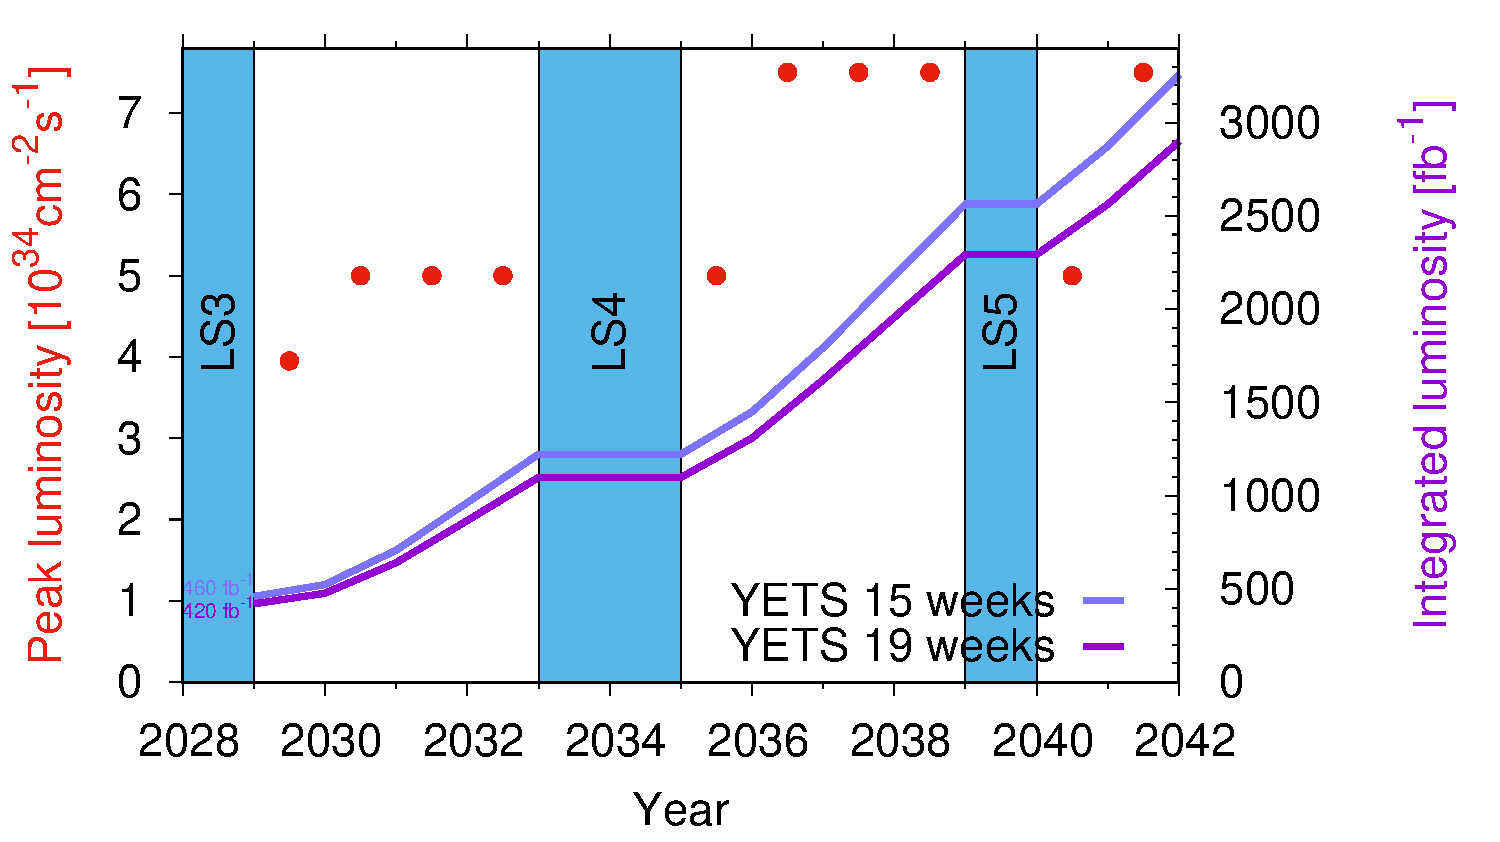
\includegraphics[width=0.8\textwidth]{figures/Part2/Upgrade/Lumi}
 \end{tabular}
 \caption{The peak and intergraded luminosity expected to be delivered by the \ac{HL-LHC}, taken from~\cite{LHC:plan} in November 2023. The left-hand $y$-axis shows the scale of the peak instantaneous luminosity, which is itself represented with red dots. The right-hand $y$-axis shows the scale of the intergraded luminosity. The two solid lines represent the intergraded luminosity under two \ac{YETS} scenarios.}
 \label{fig:Lumi}
 \end{center}
\end{figure}

An overview of the Phase-2 Upgrade is given in \autoref{sec:Overview}. Among various systems upgrades, the upgrade of the Outer Tracker is more relevant to this thesis, which is described in \autoref{sec:OT}. The Outer Tracker upgrade will enable tracking at the \ac{L1} trigger, which is discussed in \autoref{sec:Algo}. The tracking information can be combined with the calorimeter responses to build electron candidates at the \ac{L1} trigger, which is discussed in \autoref{sec:L1Ele}.

\section{Overview of the Upgrade}
\label{sec:Overview}

A new silicon tracker~\cite{CMS:2017lum} will replace the current tracker for the Phase-2. The Phase-2 tracker is divided into two subsystems: a pixel detector known as the Inner Tracker and the Outer Tracker composed of strip and macro-pixel sensors. The Phase-2 Tracker will provide efficient tracking up to $|\eta|~<$ 4 because of the extended coverage of the Inner Tracker. The Phase-2 tracker is much lighter with improved radiation hardness while enjoying a reduced material budget in the tracking volume. The granularity of Phase-2 tracker will be increased by roughly a factor of 4, leading to a much better charged-particle $\pt$ resolution. More importantly, the Phase-2 Outer Tracker is specially designed to be capable of delivering data to the \ac{L1} trigger, which is further discussed in \autoref{sec:OT}.

The \ac{L1} trigger~\cite{Zabi:2020gjd}

The electronics of the \ac{ECAL} Barrel Calorimeter will be replaced to accomodate the \ac{L1} trigger requirements on latency and rate. The upgraded electronics will enable the Phase-2 \ac{L1} trigger to exploit the information from single crystals.

The \ac{ECAL} and \ac{HCAL} Endcap Calorimeters will be replaced by a new endcap calorimeter known as the \ac{HGCAL}~\cite{CMS:2017jpq}. The \ac{HGCAL}

The \ac{MTD}~\cite{Butler:2019rpu}

The Muon system~\cite{Hebbeker:2017bix}

The \ac{HLT} ~\cite{HLT:Upgrade}

Upgrades of the \ac{BRIL} system is also planned and is documented in details in Ref.~\cite{Beam:Upgrade}.

\section{The Outer Tracker Upgrade}
\label{sec:OT}

The trigger primitives produced by the Outer Tracker, known as ``stubs'', form input to the track finding algorithm. The initial stage of the algorithm involves correlating stubs from two adjacent layers to form ``tracklets''. The tracklets are then used as seeds for extrapolating to other layers and disks to match with additional stubs. A \ac{KF} takes all potential tracks from combinations of tracklet and stubs, and produces the best track fit.

\begin{figure}[tbh!]
 \begin{center}
  \begin{tabular}{c}
   \centering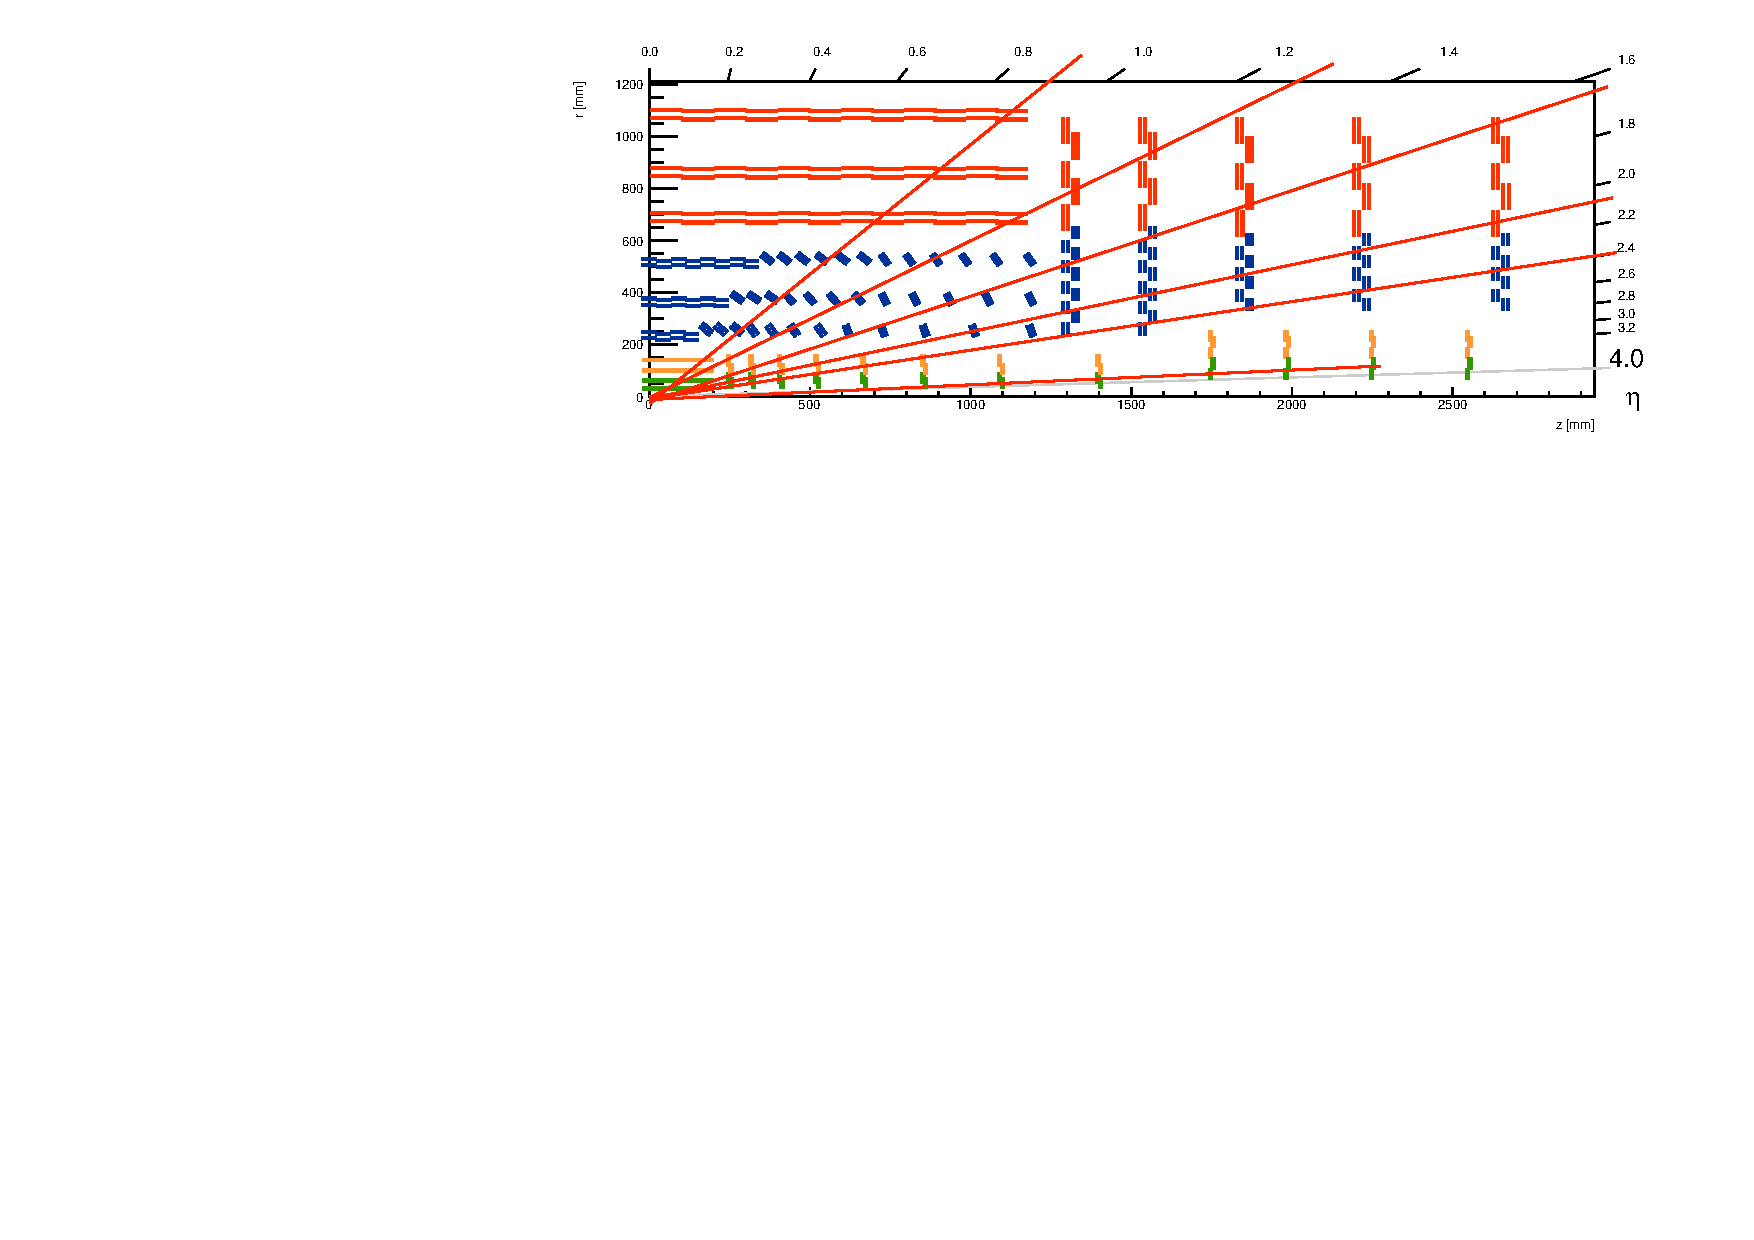
\includegraphics[width=0.9\linewidth]{figures/Part2/Upgrade/TrackerGeo}
  \end{tabular}
  \caption{(Layout of one quadrant of the Phase-2 \ac{CMS} tracker in the $r-z$ plane, generated by the \ac{CMSSW}~\cite{cmssw}. The PS modules of the Outer Tracker are represented with blue lines while the 2S modules are represented with red lines. The inner tracker modules are represented with orange and green lines, which do not contribute to the \ac{L1} trigger.}
 \label{fig:TrackerGeo}
 \end{center}
\end{figure}

The trigger primitives produced by the Outer tracker, known as ``stubs'', form input to the track finding algorithm. The initial stage of the algorithm involves correlating stubs from two adjacent layers to form ``tracklets''. The tracklets are then used as seeds for extrapolating to other layers and disks to match with additional stubs. A \ac{KF} takes all potential tracks from combinations of tracklet and stubs, and produces the best track fit.

The trigger primitives produced by the Outer tracker, known as ``stubs'', form input to the track finding algorithm. The initial stage of the algorithm involves correlating stubs from two adjacent layers to form ``tracklets''. The tracklets are then used as seeds for extrapolating to other layers and disks to match with additional stubs. A \ac{KF} takes all potential tracks from combinations of tracklet and stubs, and produces the best track fit.

\begin{figure}[tbh!]
 \begin{center}
  \begin{tabular}{c}
   \centering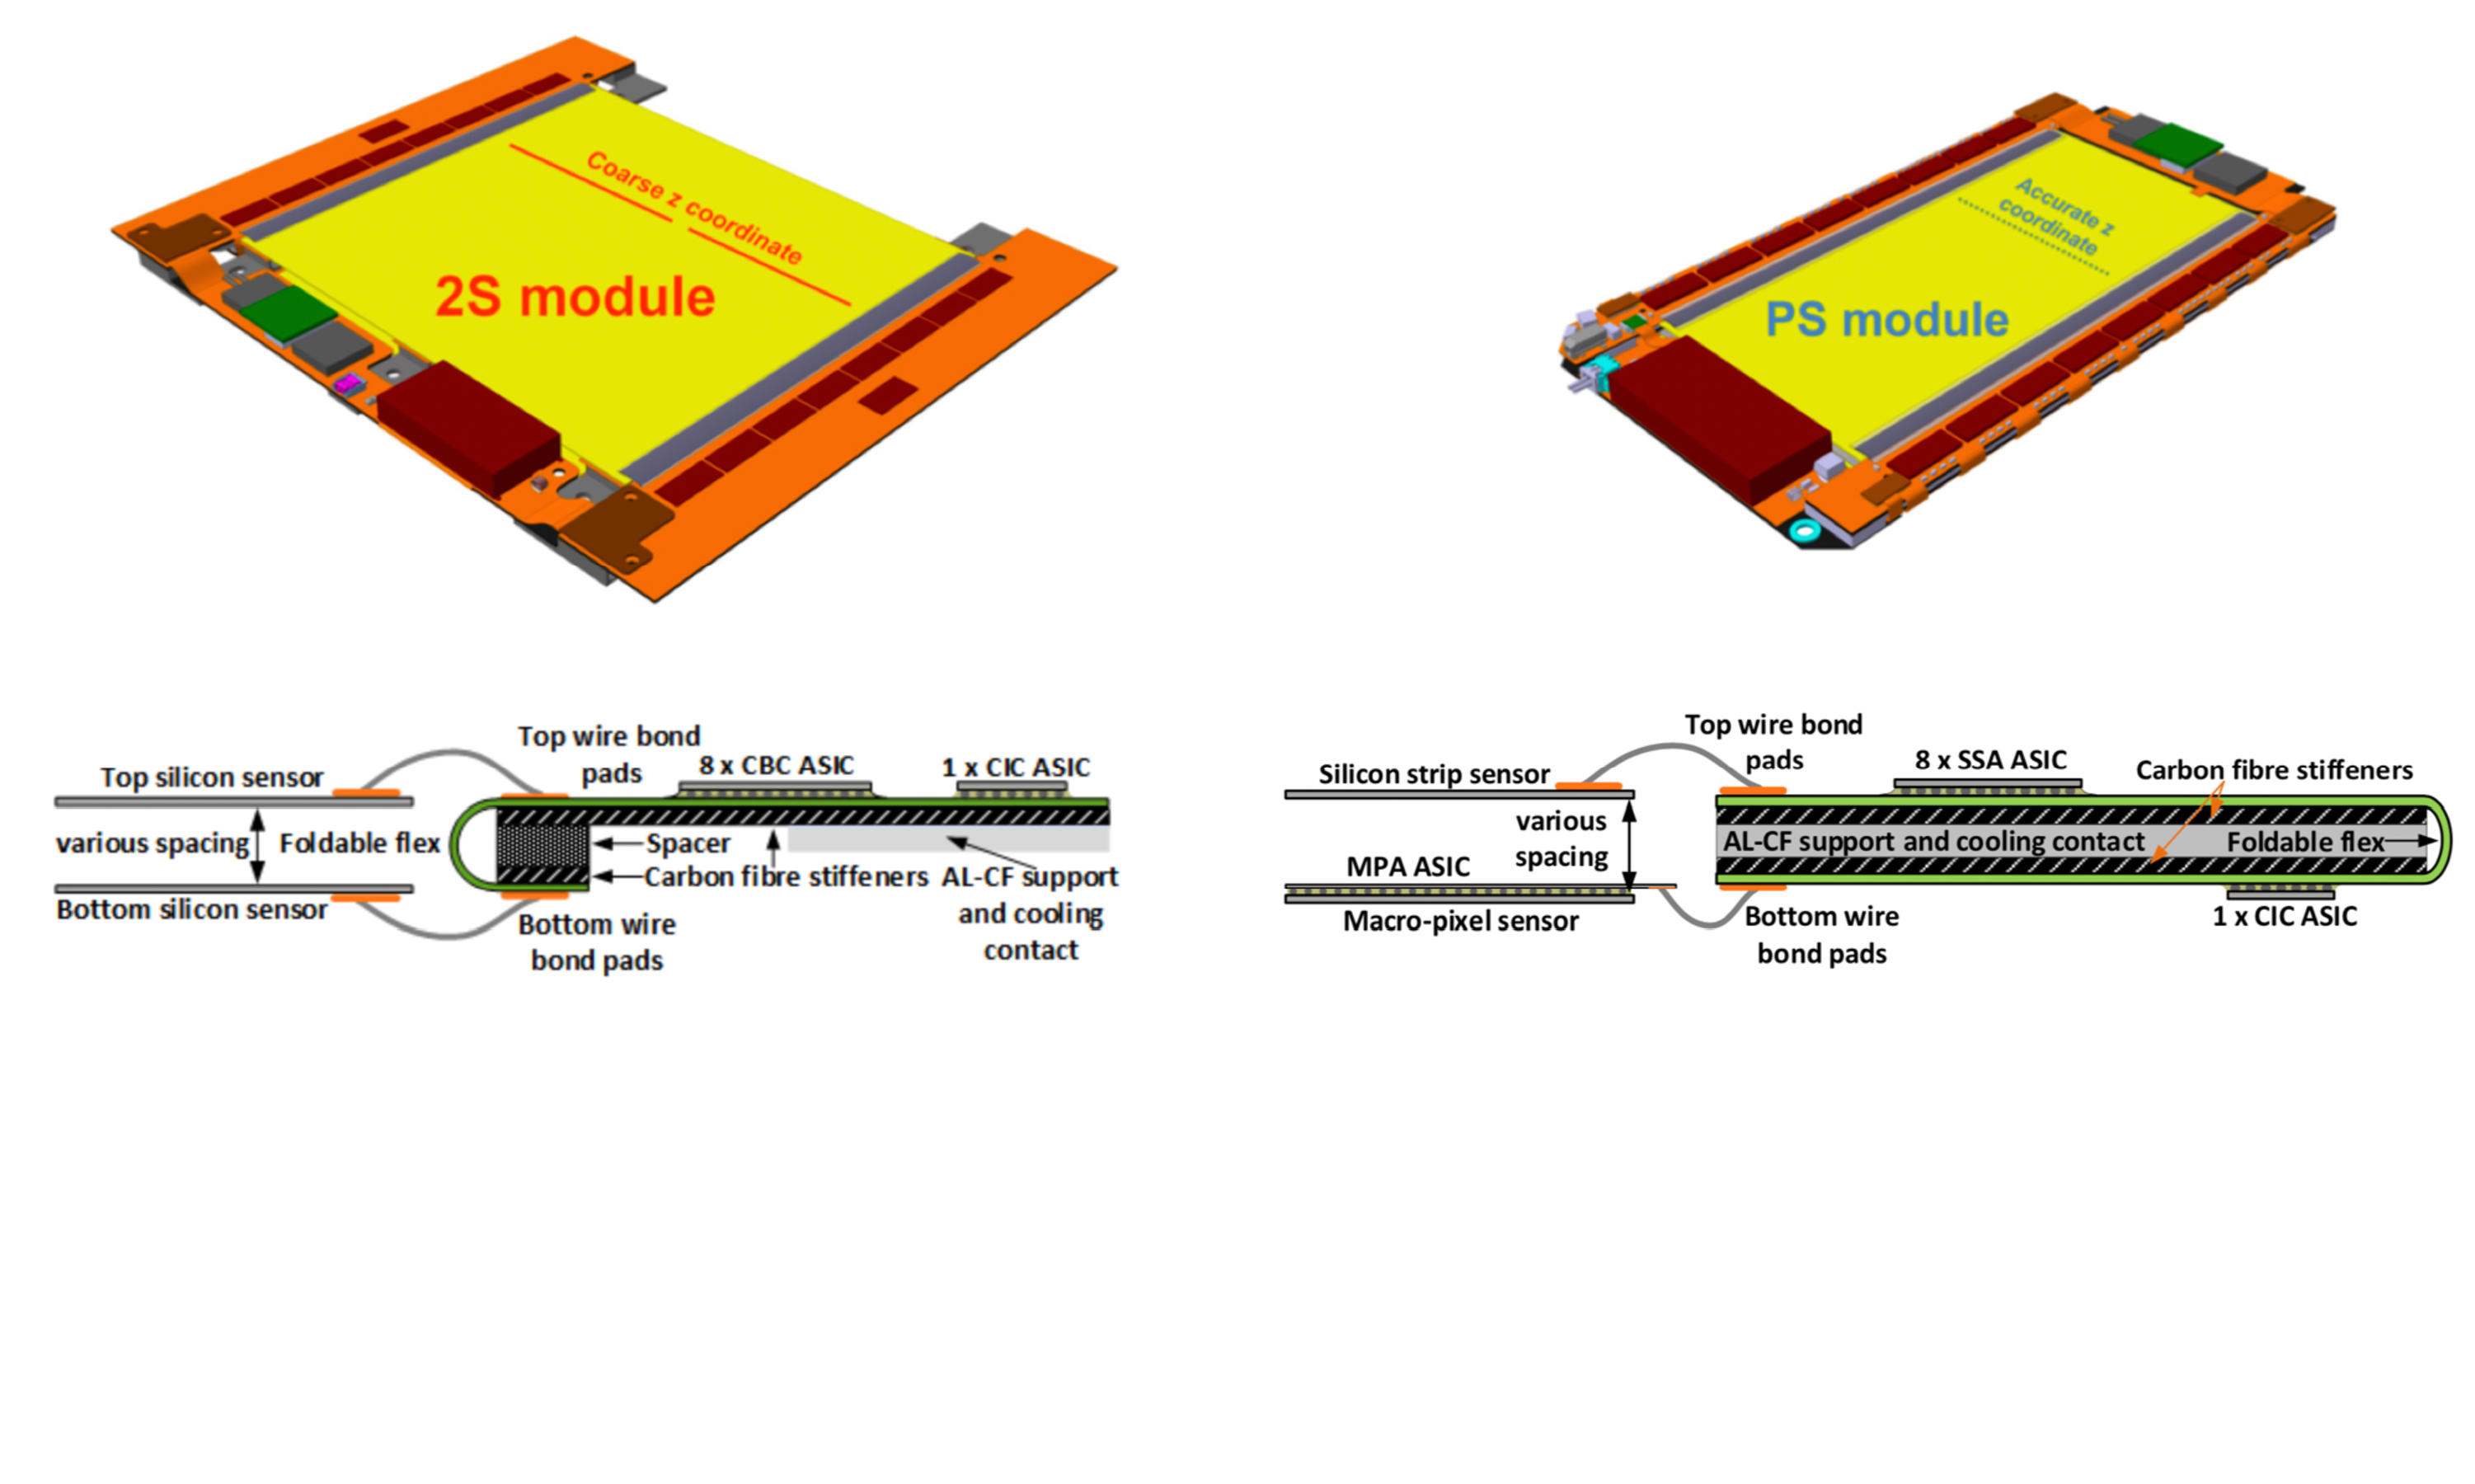
\includegraphics[width=0.95\linewidth]{figures/Part2/Upgrade/Modules}
  \end{tabular}
  \caption{Illustrations of the 2S module (left) and PS module (right), adapted from~\cite{CMS:2017lum}. Shown are views of the assembled modules (top) and  sketches of the frontend hybrid folded assembly and connectivity (bottom).}
 \label{fig:Modules}
 \end{center}
\end{figure}

To maintain a low trigger threshold even with the harsh environment, the CMS experiment is planning to replace its entire Level-1 (L1) trigger system. One of the key goals of the L1 trigger upgrade is to incorporate tracking information of the charged particles. This goal also drives the design of the Outer Tracker at \ac{HL-LHC}, which utilizes the $\pt$ modules (See Figure \ref{fig:TrackerGeo}) to produce ``trigger primitive'' for the reconstruction of the trajectories of charged particles (known as ``tracks''). Each $\pt$ module consists of two closely spaced silicon sensors. By correlating hits from two layers, the $\pt$ modules are capable of providing $\pt$ discrimination at the front end. With current design, only hits over a threshold of 2 GeV will be read out. 

\begin{figure}[tbh!]
 \begin{center}
  \begin{tabular}{cc}
   \centering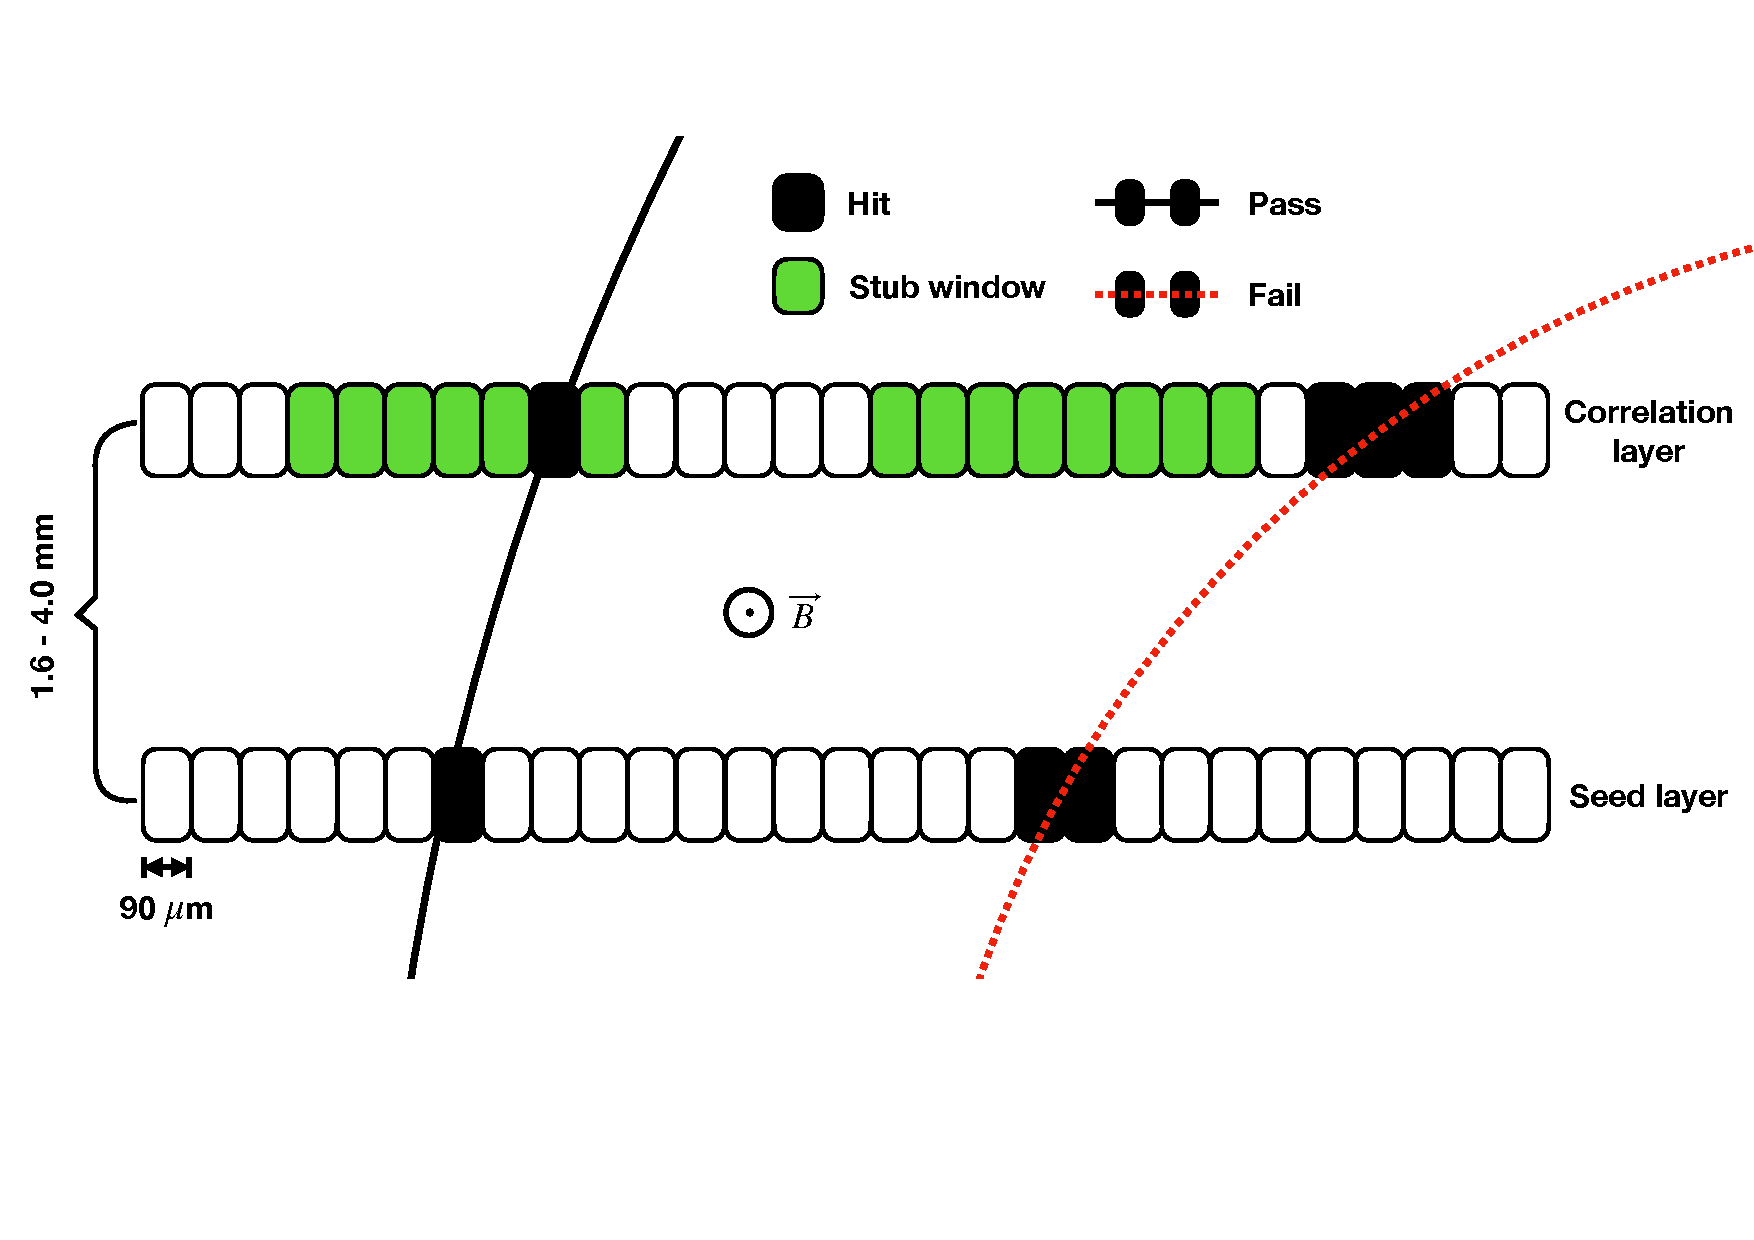
\includegraphics[width=0.9\linewidth]{figures/Part2/Upgrade/Stub}
  \end{tabular}
  \caption{(Left) Tracker geometry at the \ac{HL-LHC}. Outer Tracker consists of over 3000 $\pt$ modules. (Right) Cross section of the $\pt$ module.}
 \label{fig:Stub}
 \end{center}
\end{figure}

\section{Leve-1 Track Finder}
\label{sec:Algo}

The trigger primitives produced by the Outer Tracker, known as ``stubs'', form input to the track finding algorithm. The initial stage of the algorithm involves correlating stubs from two adjacent layers to form ``tracklets''. The tracklets are then used as seeds for extrapolating to other layers and disks to match with additional stubs. A \ac{KF} takes all potential tracks from combinations of tracklet and stubs, and produces the best track fit.

\begin{figure}[tbh!]
 \begin{center}
  \begin{tabular}{cc}
   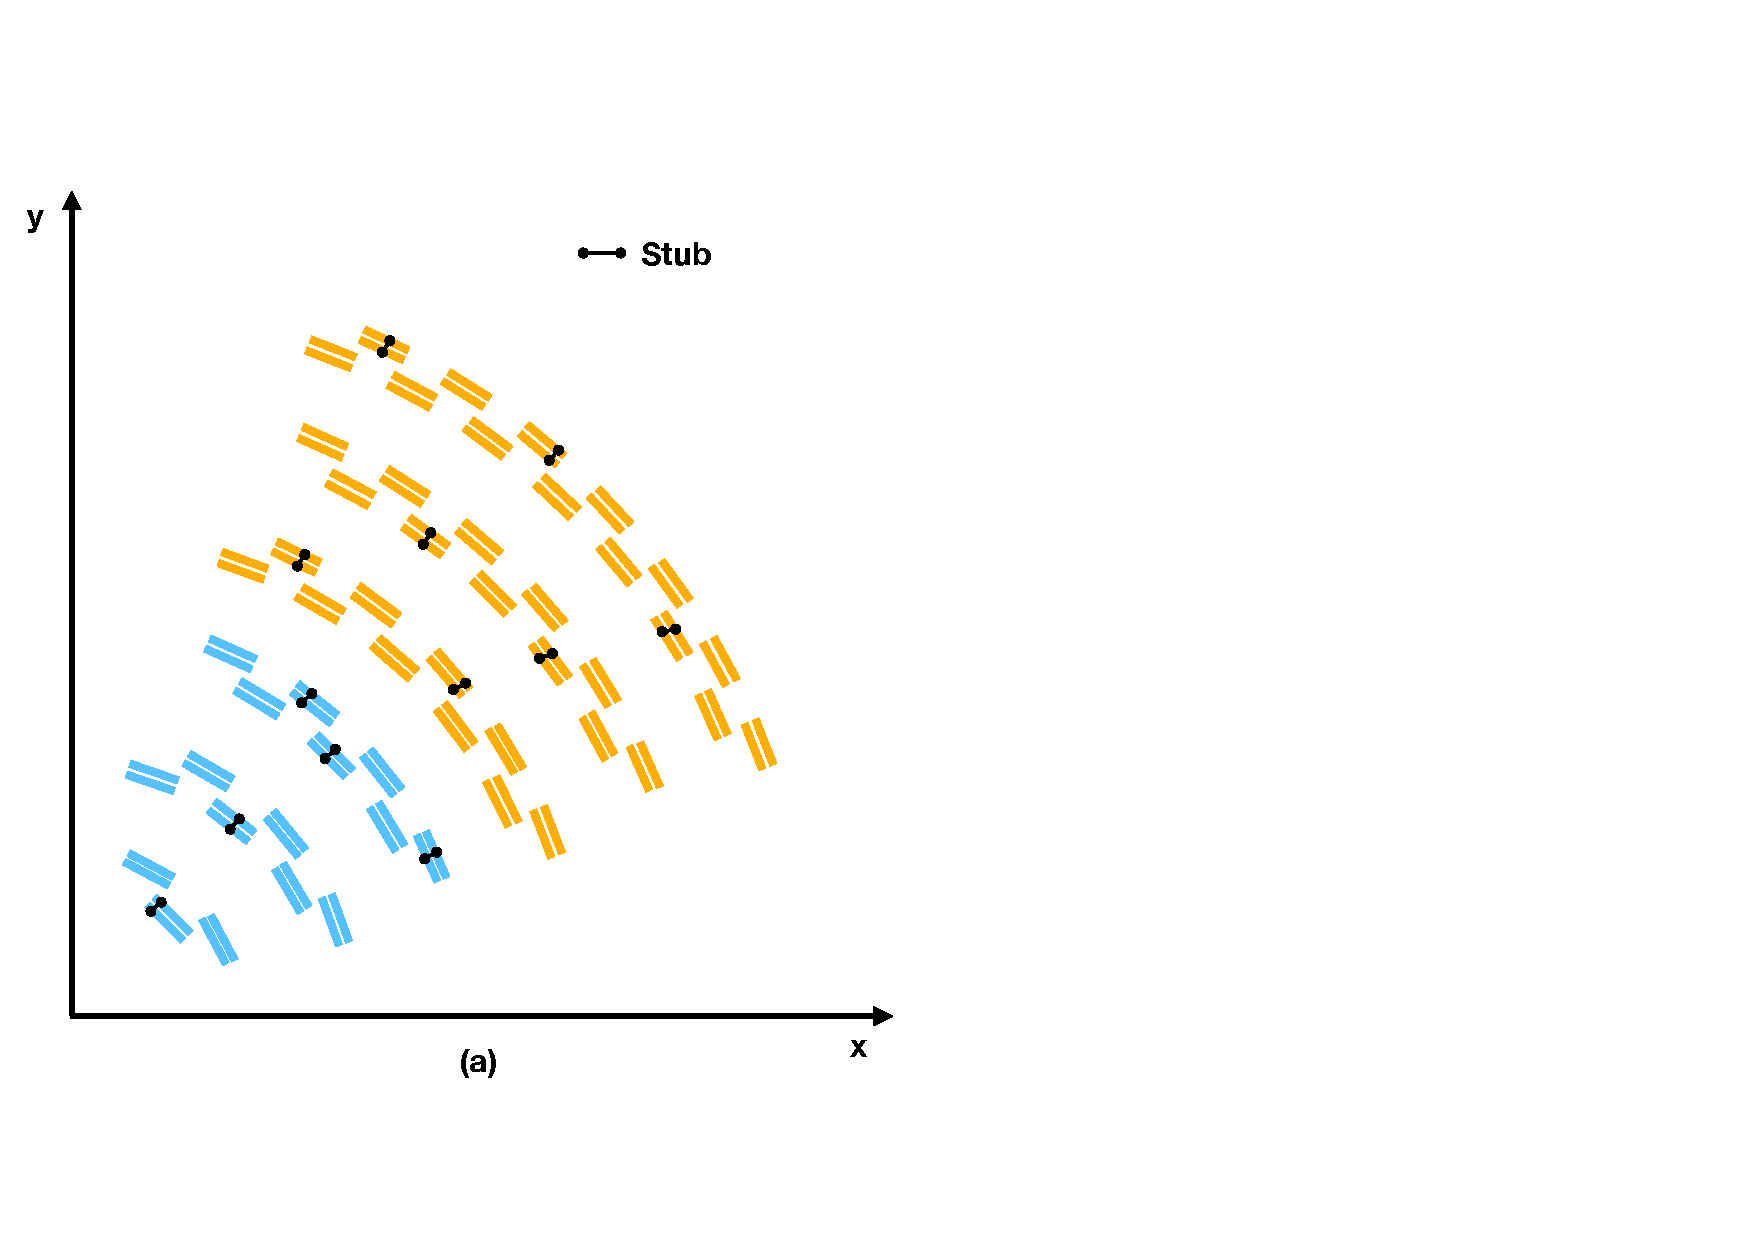
\includegraphics[width=.45\linewidth]{figures/Part2/Upgrade/tracklet1} &
   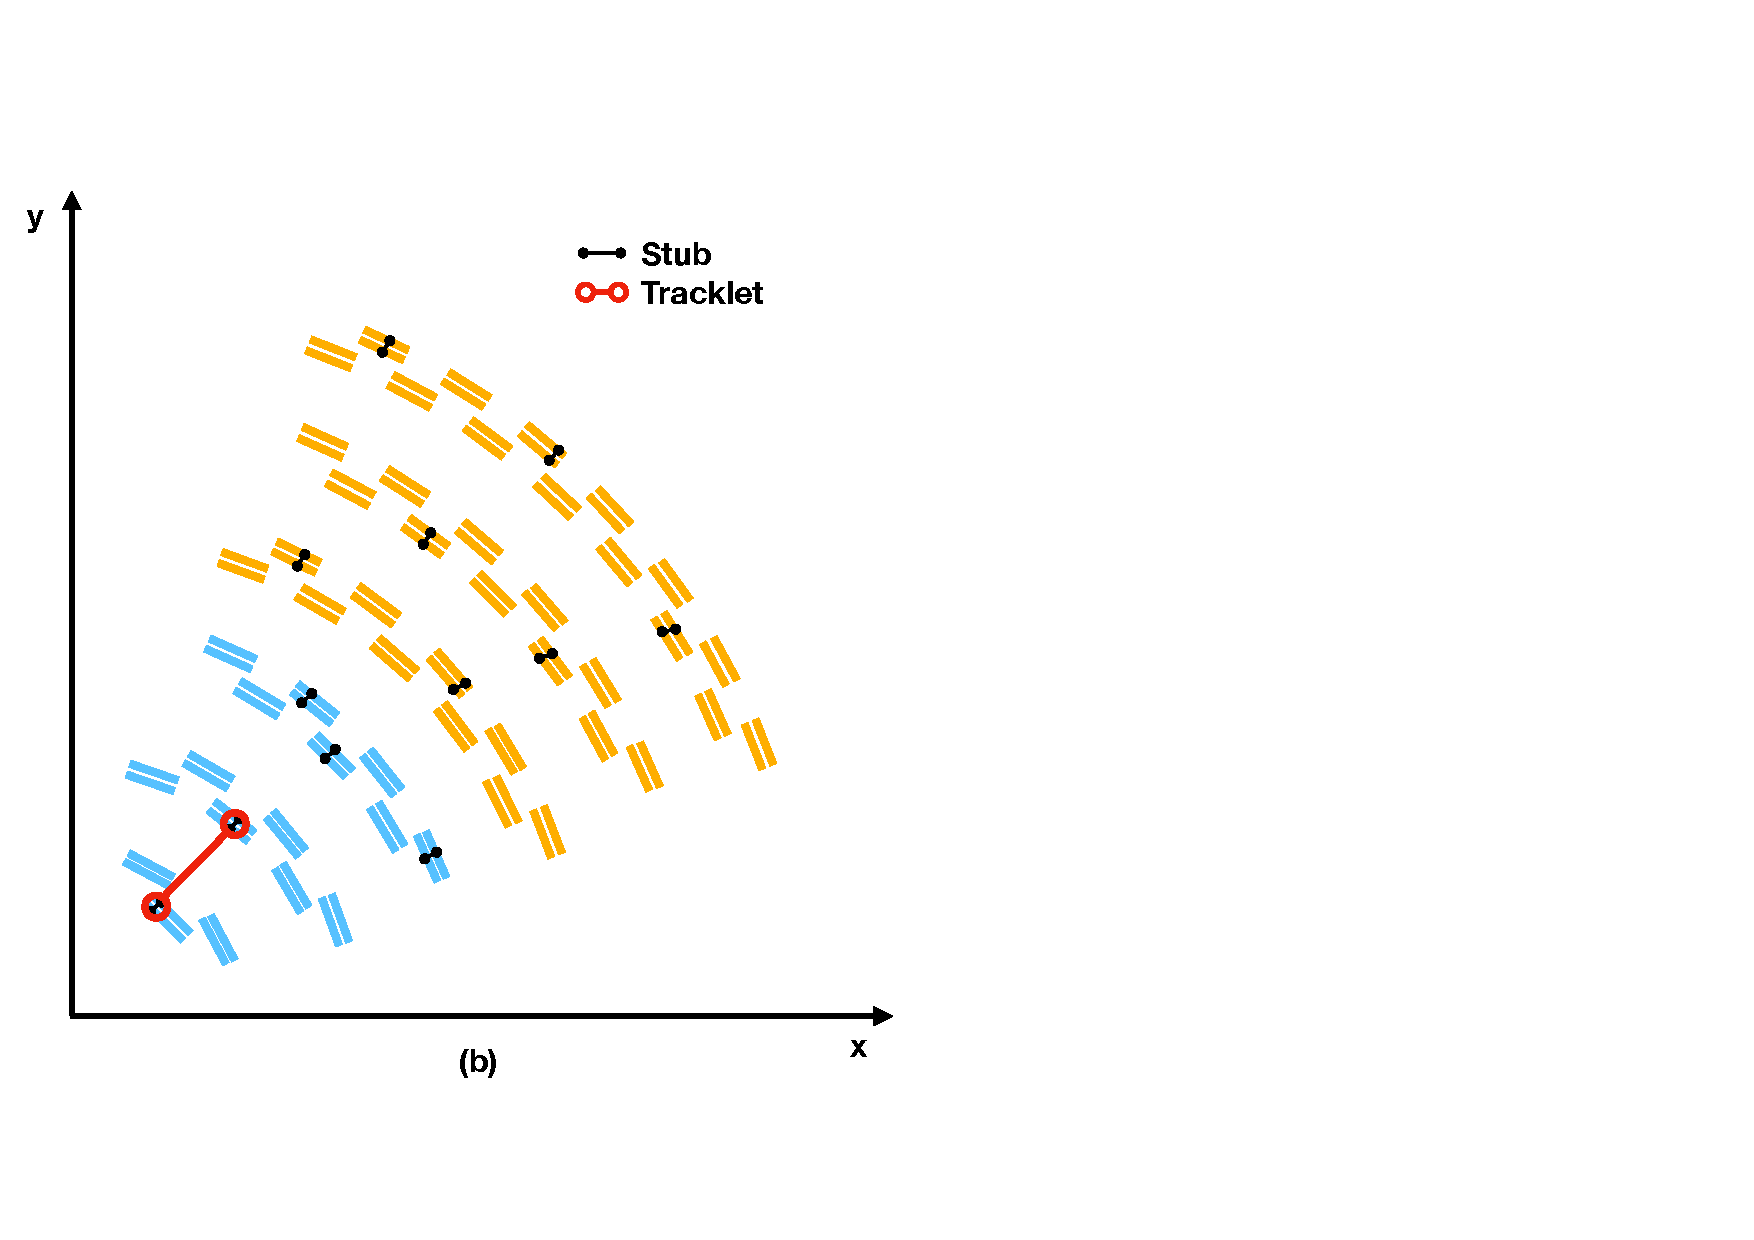
\includegraphics[width=.45\linewidth]{figures/Part2/Upgrade/tracklet2} \\
   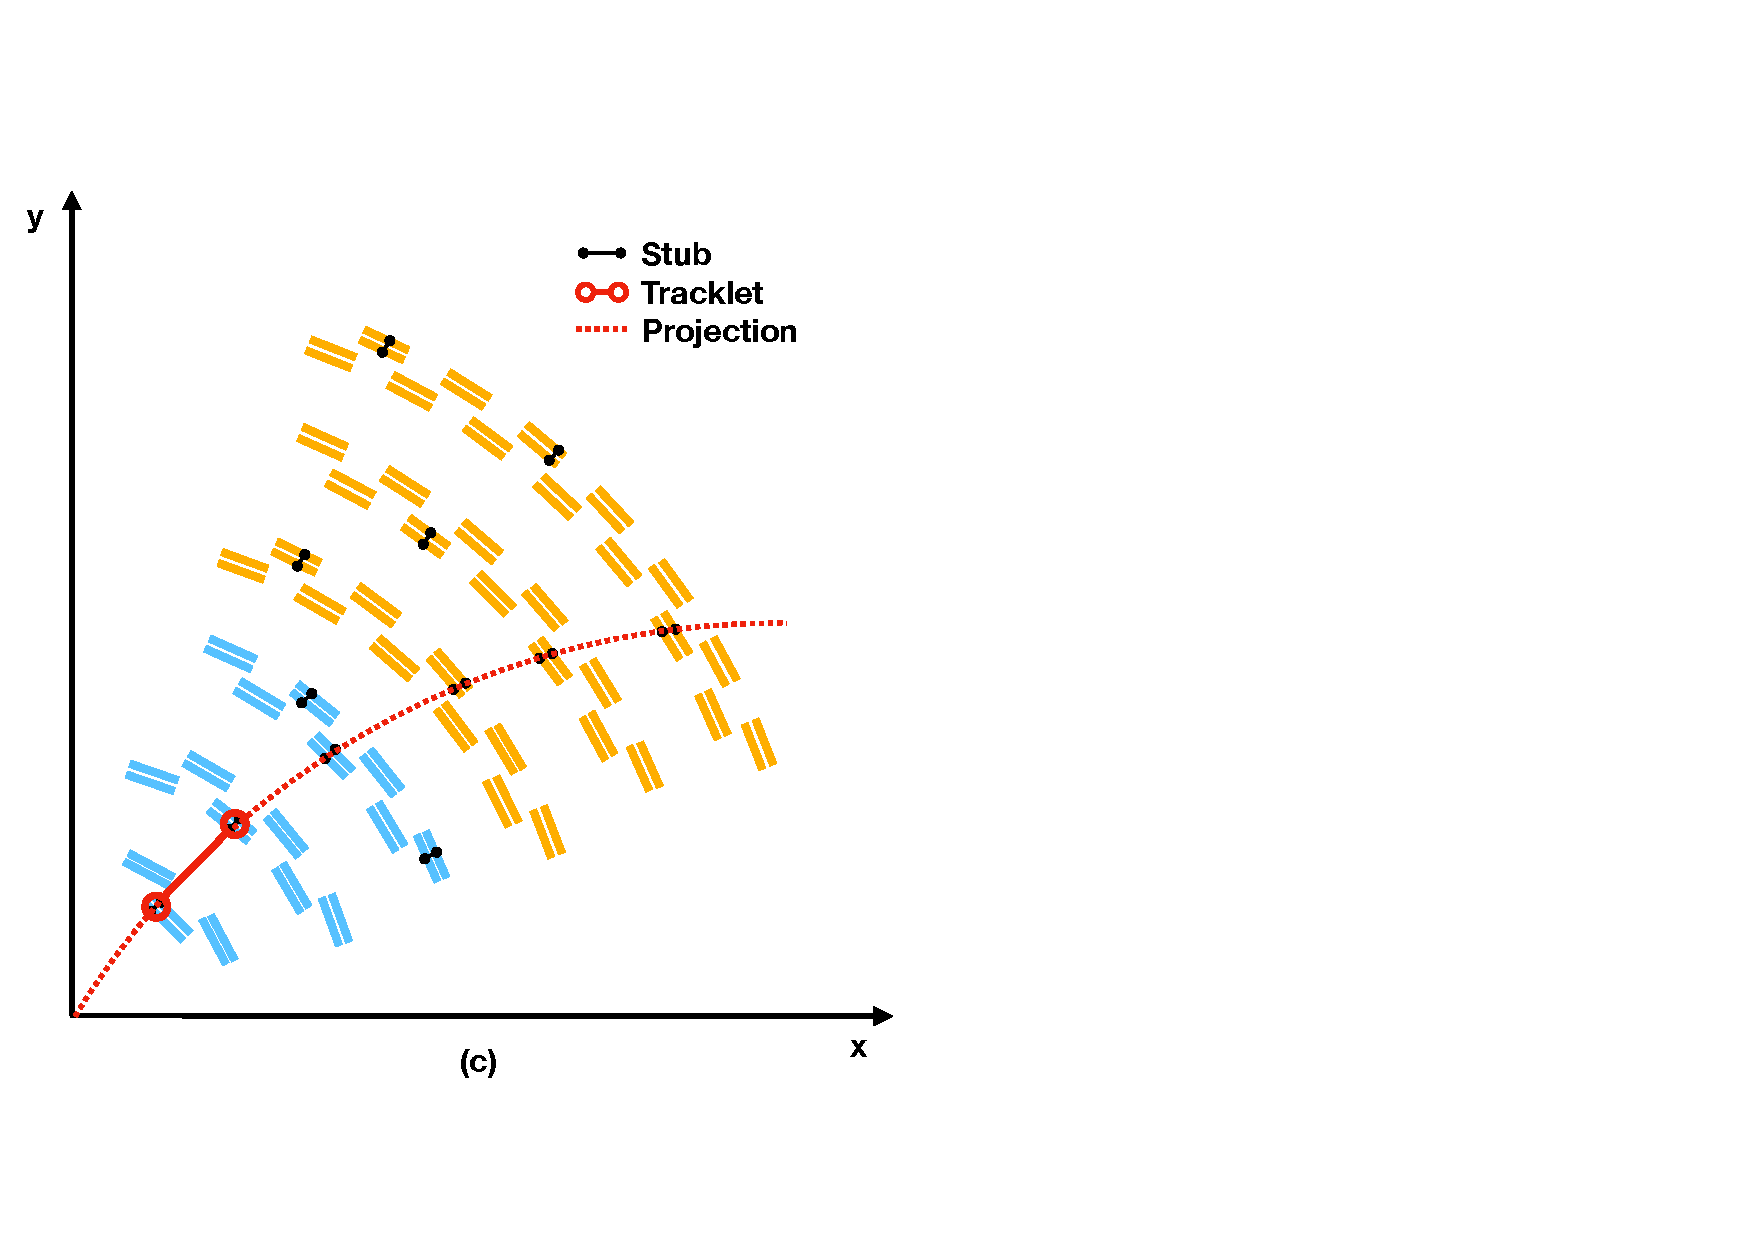
\includegraphics[width=.45\linewidth]{figures/Part2/Upgrade/tracklet3} &
   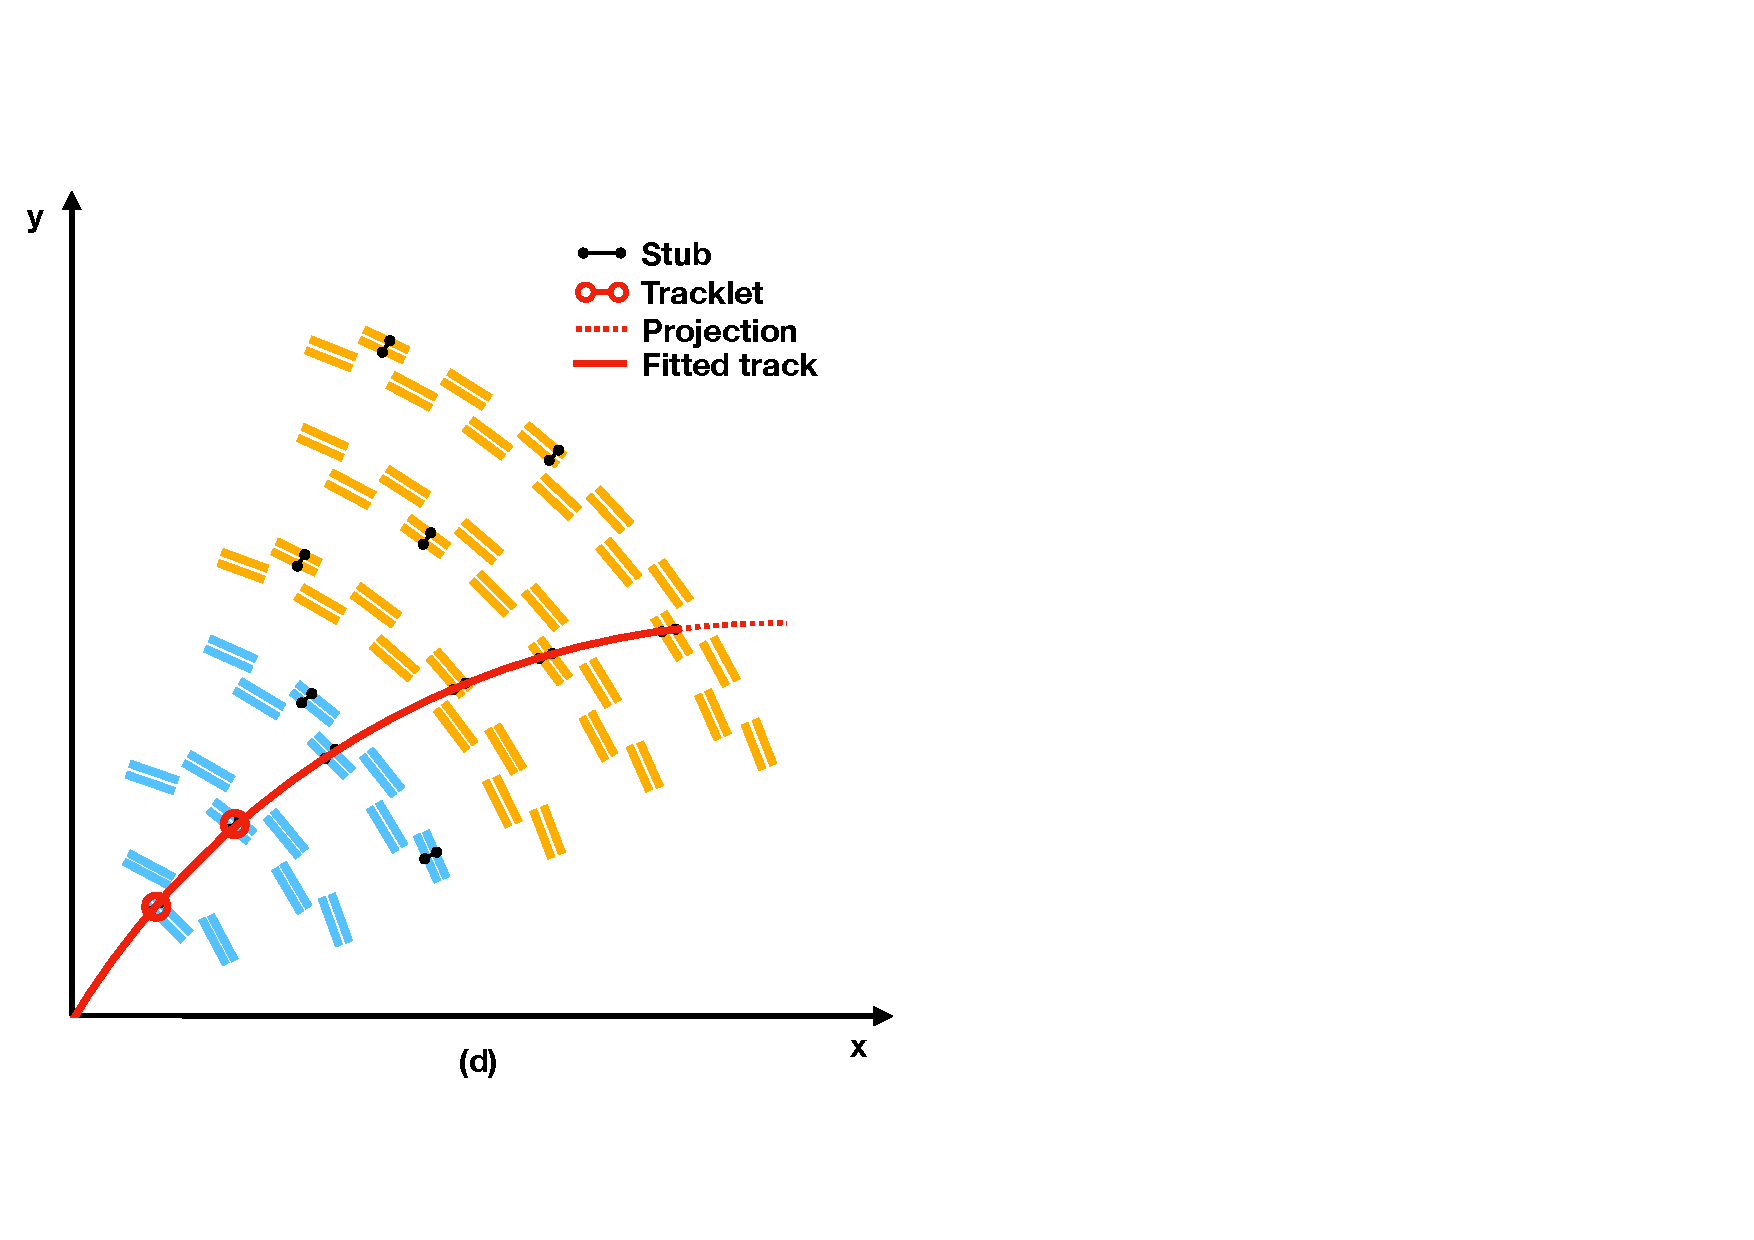
\includegraphics[width=.45\linewidth]{figures/Part2/Upgrade/tracklet4} \\
  \end{tabular}
  \caption{Illustration of different stages of the track finding algorithm: (a) constructing stubs, (b) forming tracklet by correlating two stubs and the beam spot (origin), (c) projecting to other layers and finding matches, and (d) fitting track parameters.}
 \label{fig:algorithm}
 \end{center}
\end{figure}

The baseline version of the algorithm requires at least four stubs and constrains the origin of the trajectories to the beam spot. An ``extended'' version of the algorithm is also in development, in which the beam spot constraint is relaxed. 

The track finding algorithm has demonstrated a robust performance (See Figure \ref{fig:trackingperformance}) in software simulation and is currently being tested on physical hardware. The project is progressing well and is on track for delivery before the start of the \ac{HL-LHC} in 2029. 

 \begin{figure}[tbh!]
 \begin{center}
  \begin{tabular}{cc}
   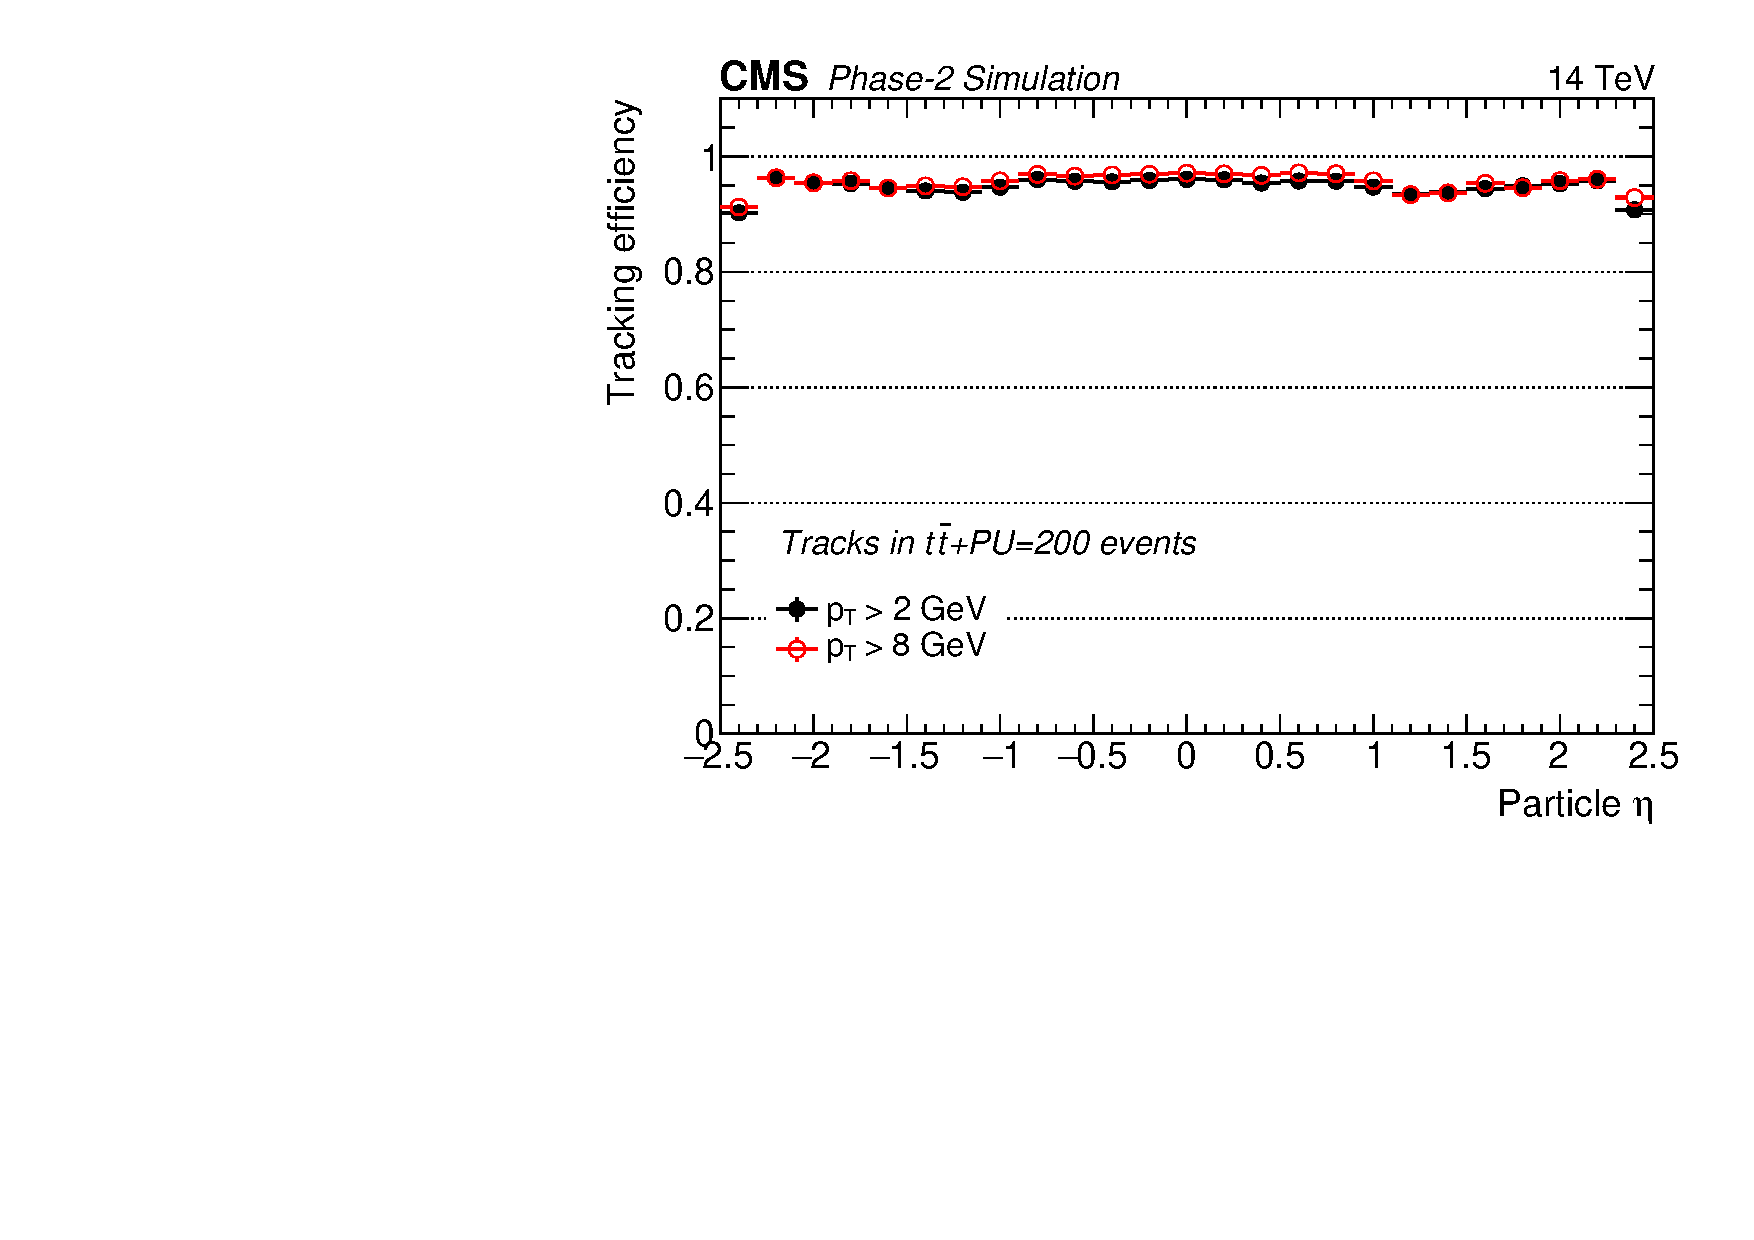
\includegraphics[width=.45\linewidth]{figures/Part2/Upgrade/L1TK_ttbar-pu200_eff_eta}&
   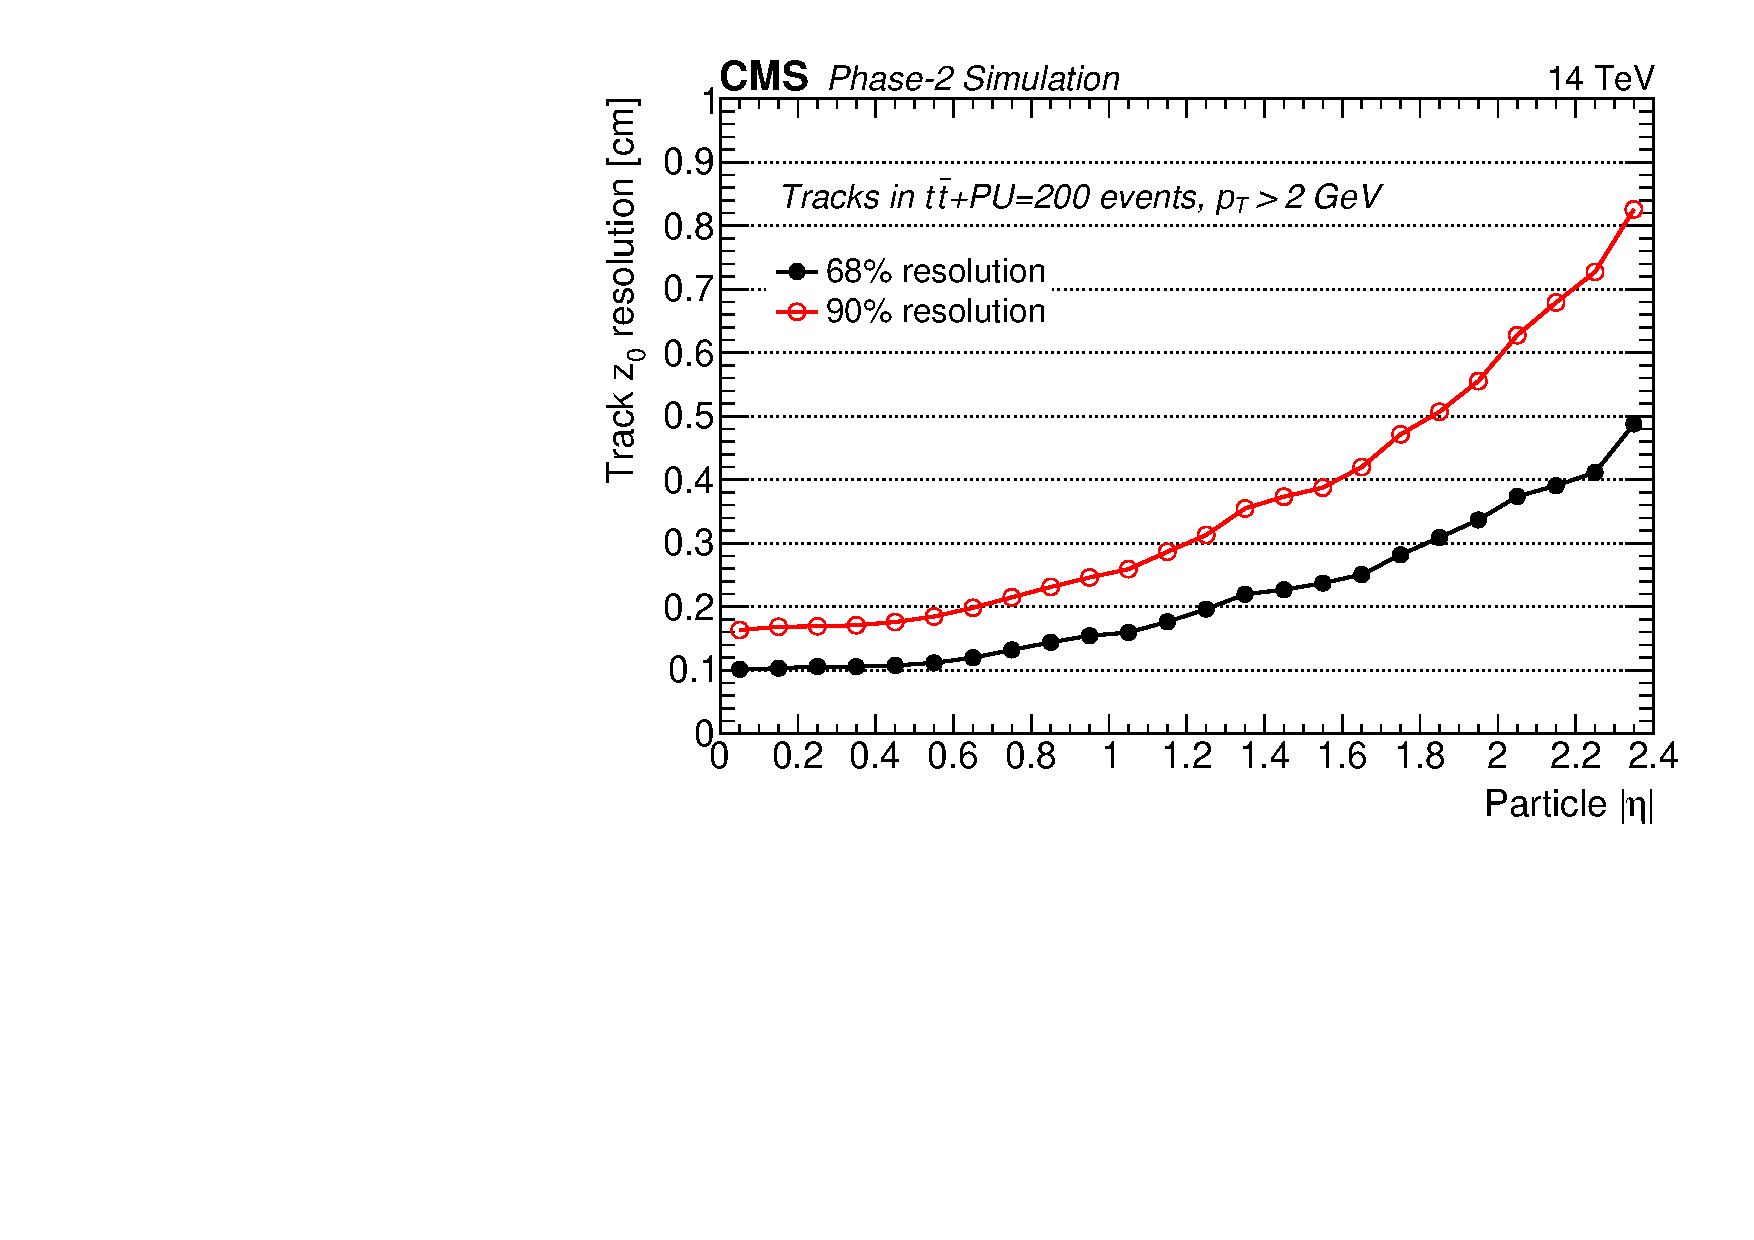
\includegraphics[width=.45\linewidth]{figures/Part2/Upgrade/L1TK_ttbar-pu200_resVsEta_z0}
  \end{tabular}
  \caption{(Left) Tracking efficiency vs particle $\eta$, measured in $\ttbar$ samples. (Center) Track $z_0$ resolution vs particle $\eta$. (Right) Electron tracking efficiency vs particle $\eta$.}
 \label{fig:trackingperformance}
 \end{center}
\end{figure} 

 \begin{figure}[tbh!]
 \begin{center}
  \begin{tabular}{cc}
   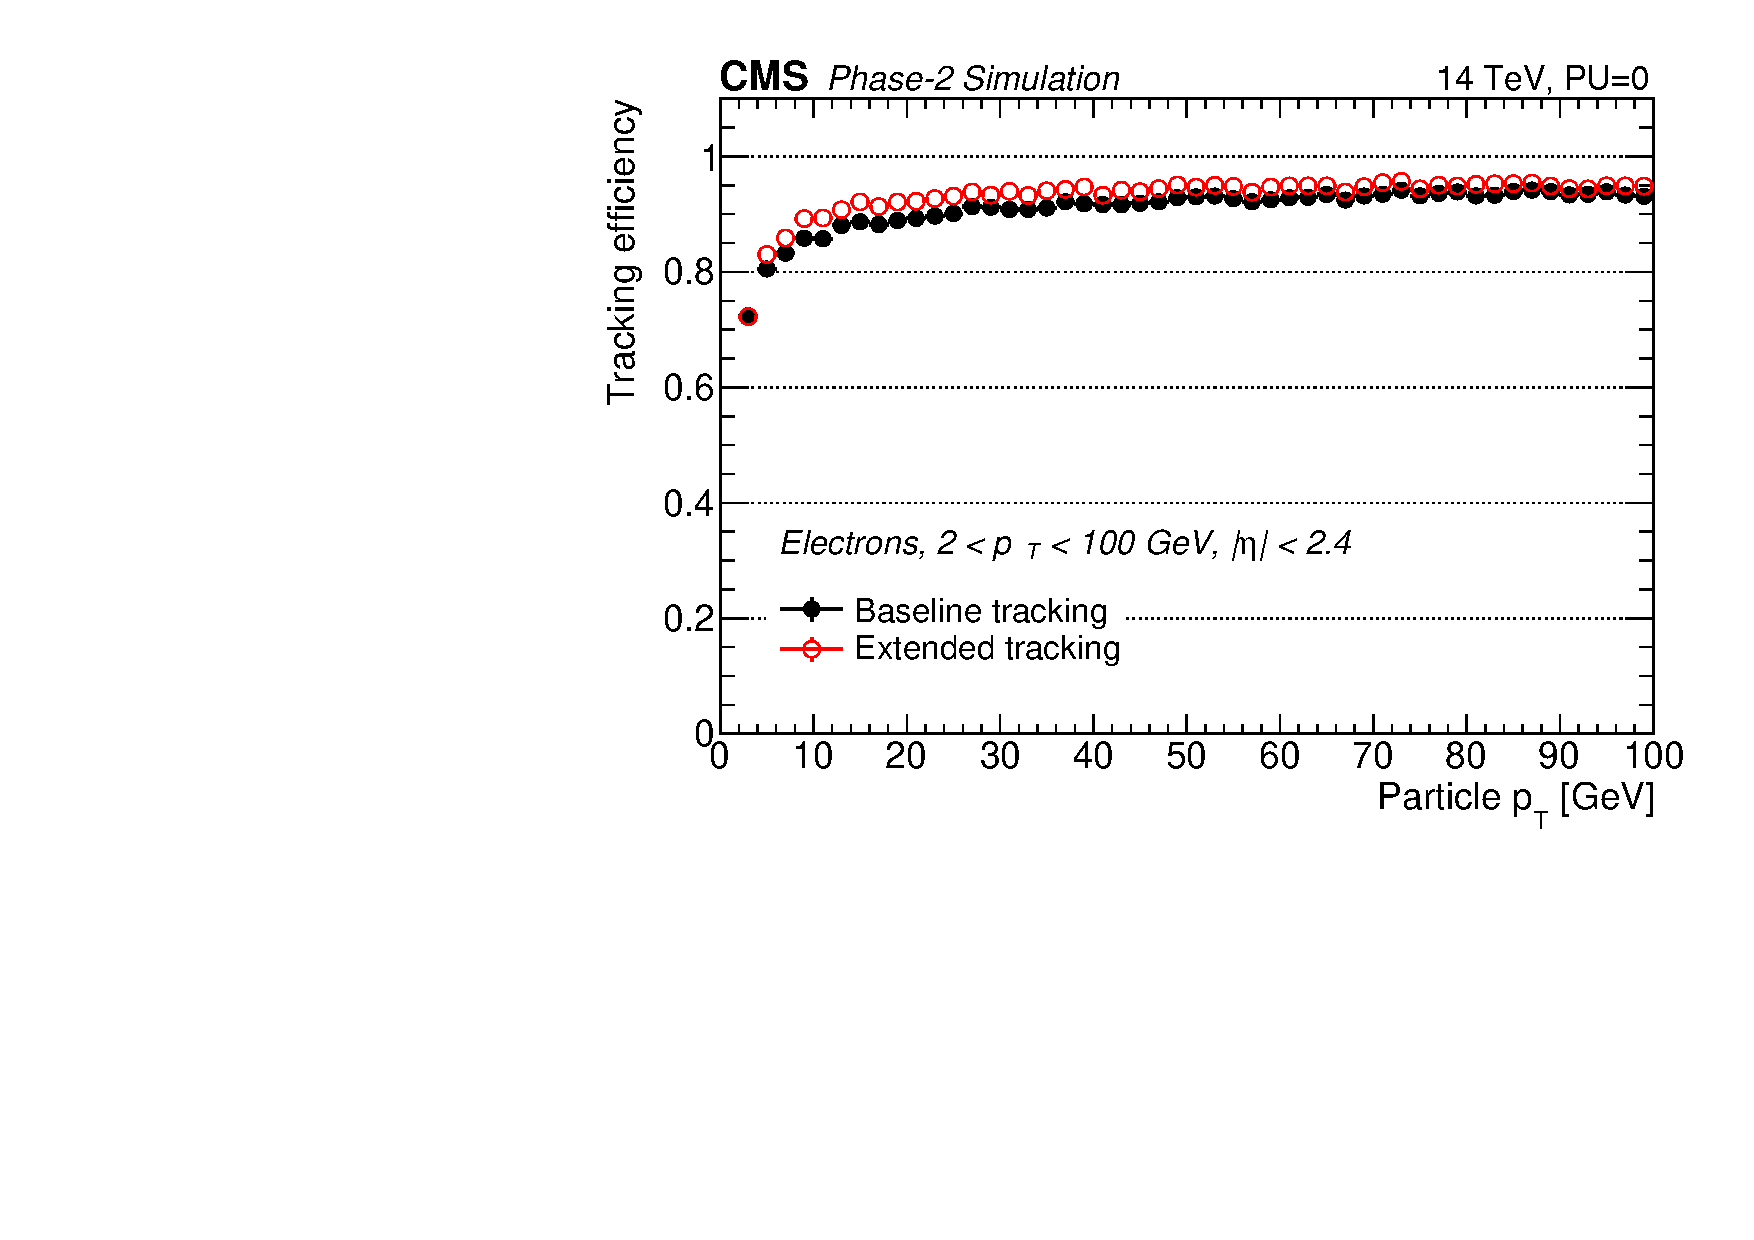
\includegraphics[width=.45\linewidth]{figures/Part2/Upgrade/L1TK_elec-pu0_eff_pt}&
   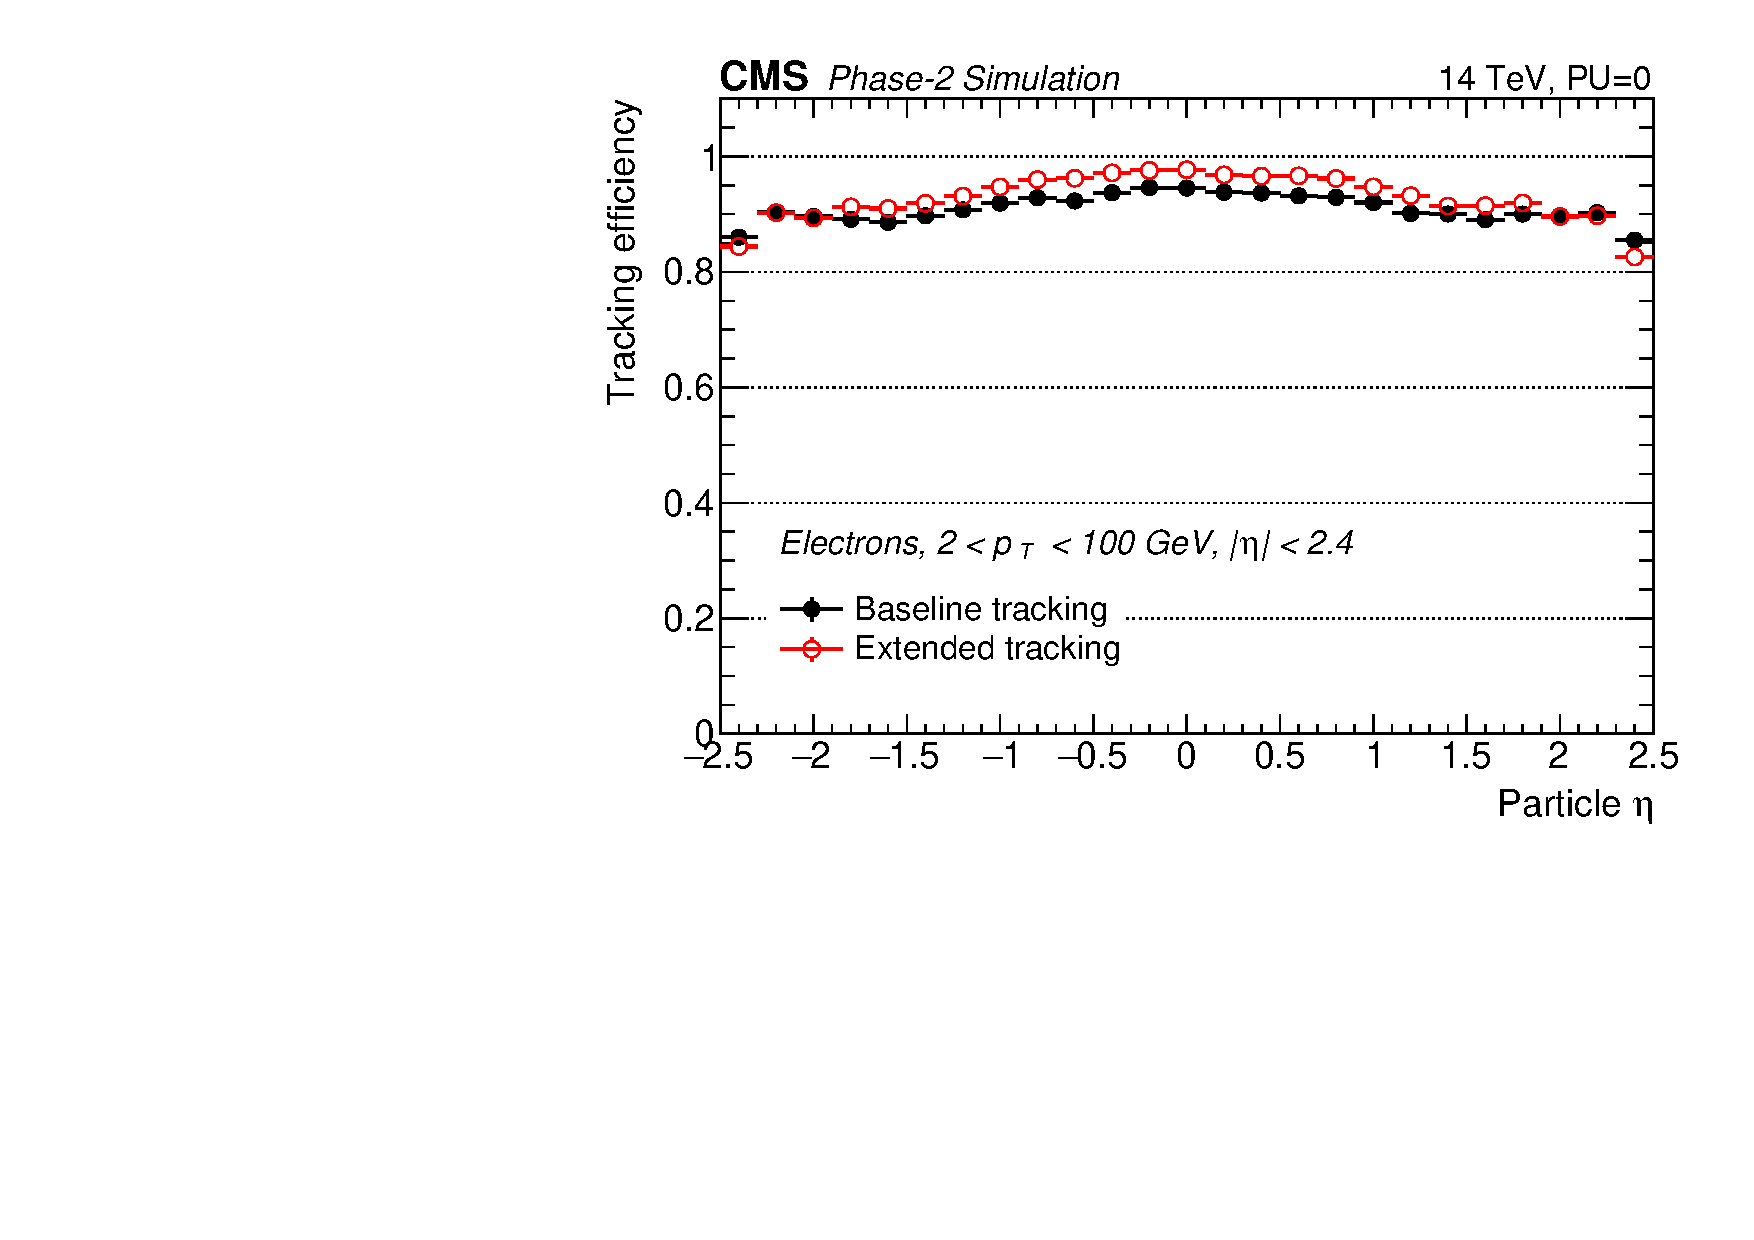
\includegraphics[width=.45\linewidth]{figures/Part2/Upgrade/L1TK_elec-pu0_eff_eta}
  \end{tabular}
  \caption{(Left) Tracking efficiency vs particle $\eta$, measured in $\ttbar$ samples. (Center) Track $z_0$ resolution vs particle $\eta$. (Right) Electron tracking efficiency vs particle $\eta$.}
 \label{fig:electronperformance}
 \end{center}
\end{figure} 

\section{Leve-1 Electron Trigger Algorithm}
\label{sec:L1Ele}

With the increase of the instantaneous luminosity, triggering on electrons will face unprecedented challenges as the data volume becomes too large to be recorded. The addition of tracking information provides a much-needed handle for the electron trigger. It enables precise track-cluster matching to lower the trigger rate. To take advantage of this new tool, a new electron trigger algorithm is developed: L1 tracks are propagated to the calorimeter surface to match with calorimeter clusters. An elliptical cut in the $\eta-\phi$ plane is applied and illustrated in Figure \ref{fig:electron} (left). Figure \ref{fig:electron} (center) demonstrates the small efficiency drop relative to the calorimeter-only algorithm. Figure \ref{fig:electron} (right) demonstrates the resulting sizable rate reduction.  
  
 \begin{figure}[tbh!]
 \begin{center}
  \begin{tabular}{ccc}
   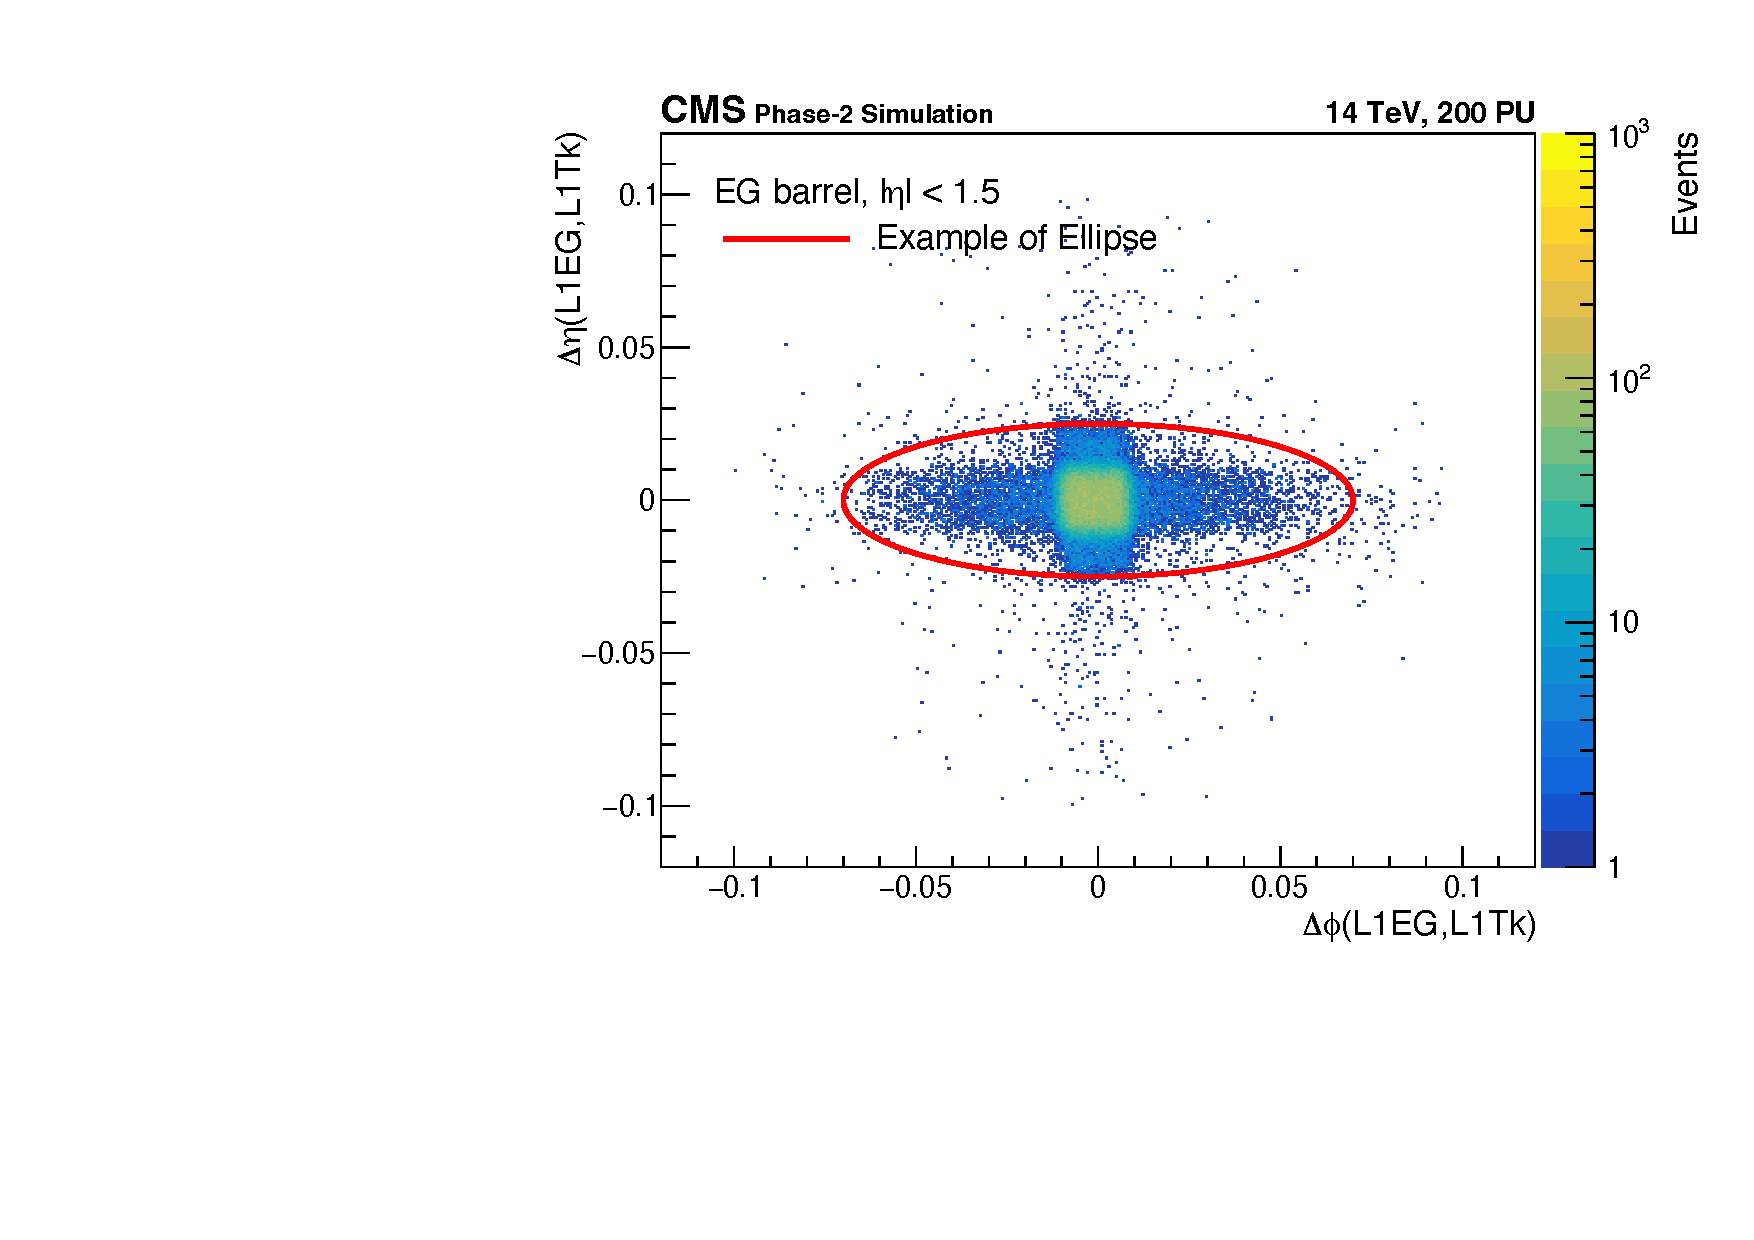
\includegraphics[width=.45\linewidth]{figures/Part2/Upgrade/DR_barrel}&
   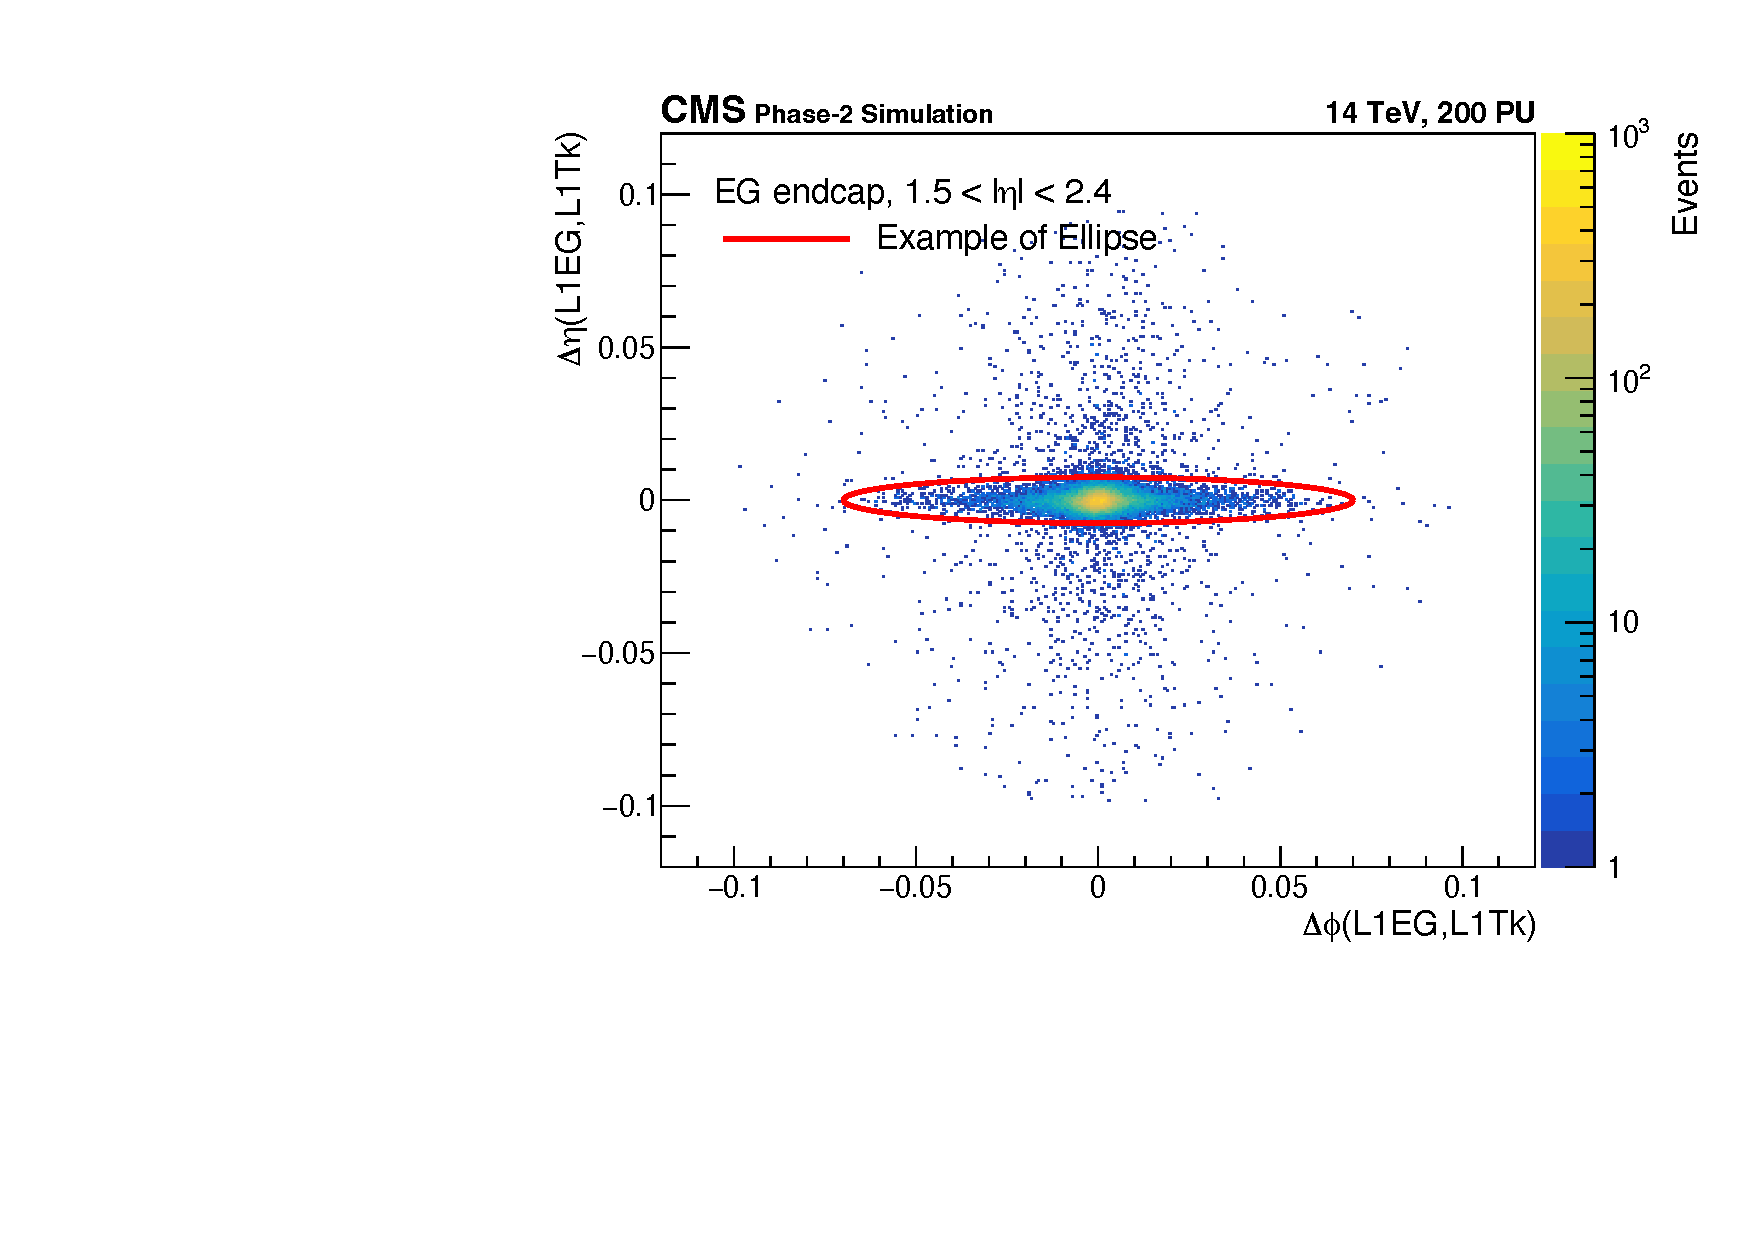
\includegraphics[width=.45\linewidth]{figures/Part2/Upgrade/DR_endcap}&
  \end{tabular}
  \caption{(Left) $\mathrm{\Delta}\eta$ vs $\mathrm{\Delta}\phi$ distances between calorimeter clusters and the closest L1 track. (Center) single electron efficiency as a function of the generated $\pt$. The efficiency drop is largely driven by electron track reconstruction which is also reflected in Figure~\ref{fig:trackingperformance}. (Right) trigger rate as a function of the cluster $\pt$.}
 \label{fig:electron}
 \end{center}
\end{figure}

When compared to the existing track-electron algorithm, this newly developed algorithm improved the electron identification efficiency by about 5$\%$ while reducing trigger rates by a factor of 2. The firmware implementation of this new algorithm is under development. Further improvement of this algorithm is possible with the ``extended'' tracking as well as a dedicated electron track quality classifier.

 \begin{figure}[tbh!]
 \begin{center}
  \begin{tabular}{ccc}
   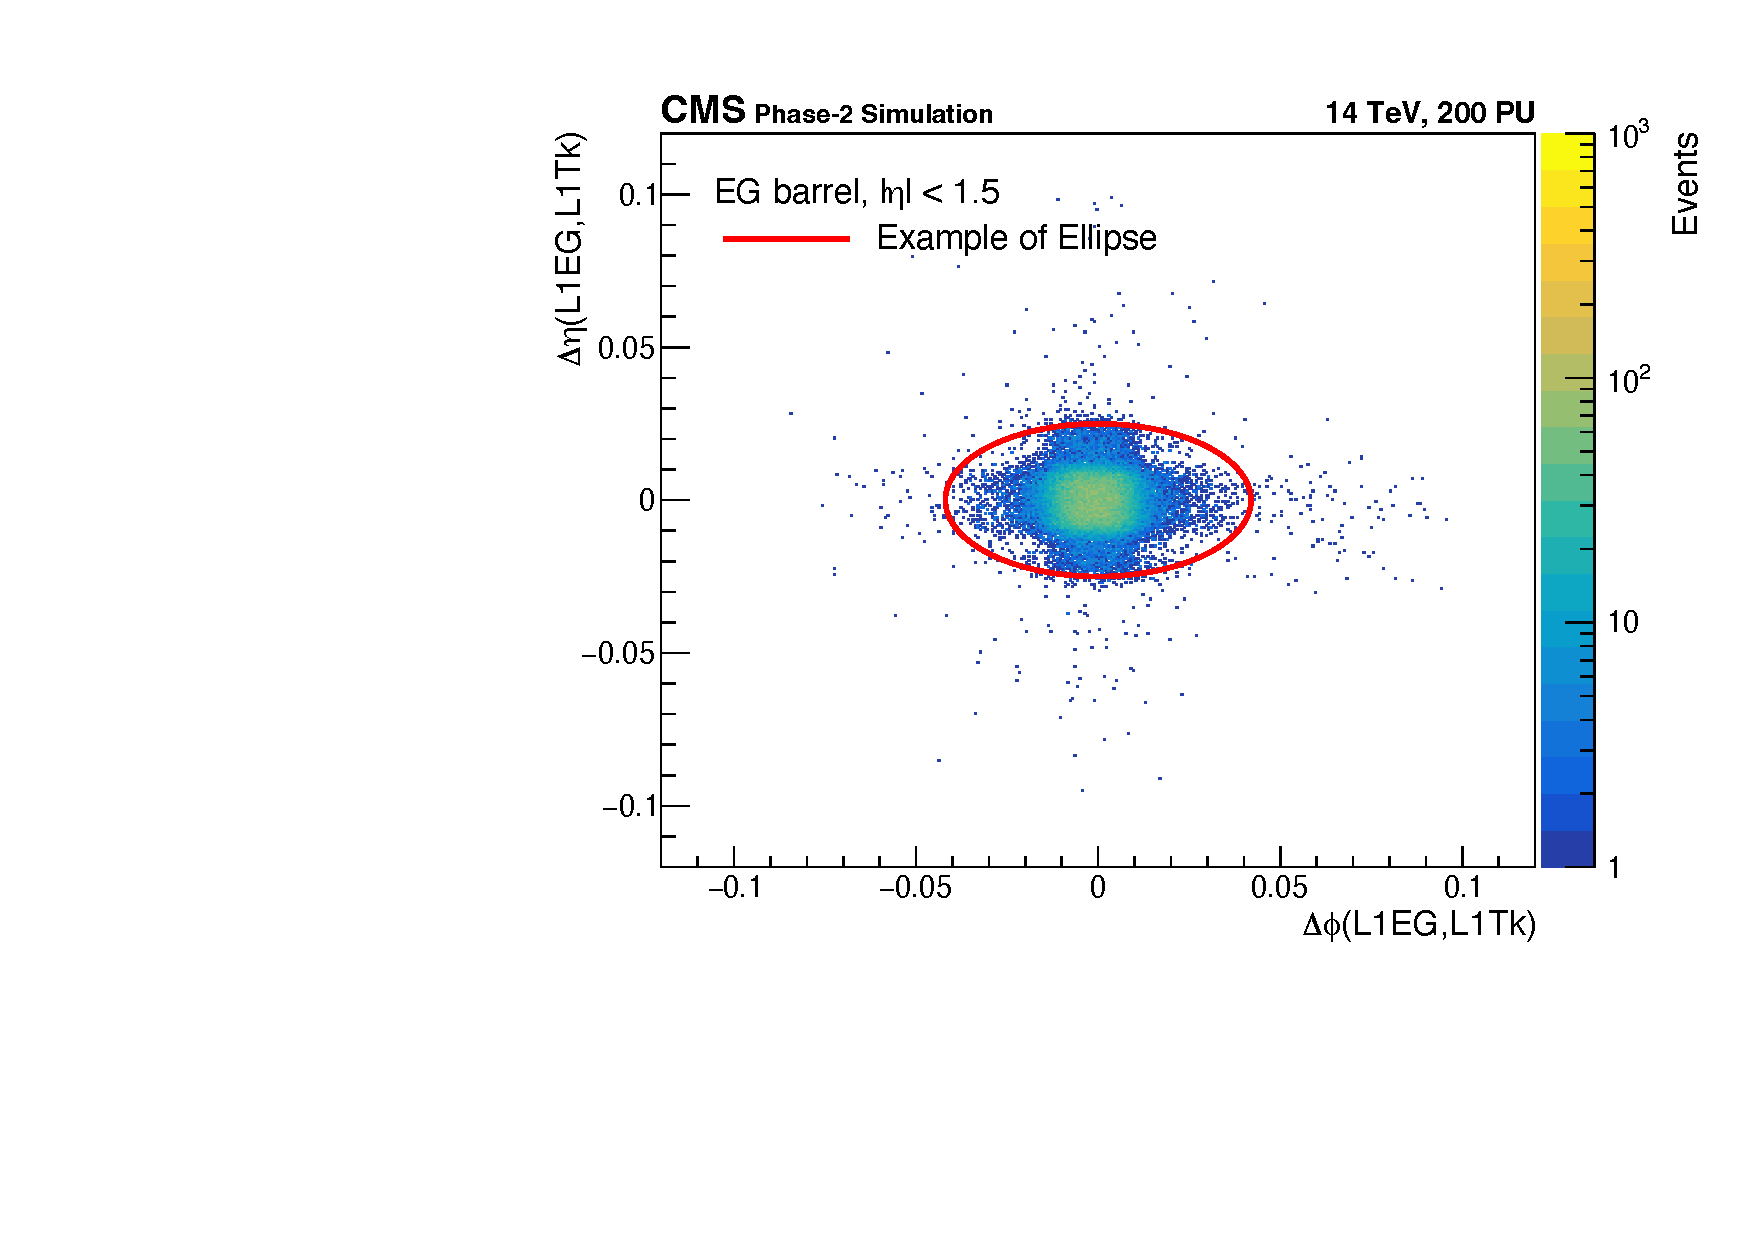
\includegraphics[width=.45\linewidth]{figures/Part2/Upgrade/DR_barrel_new}&
   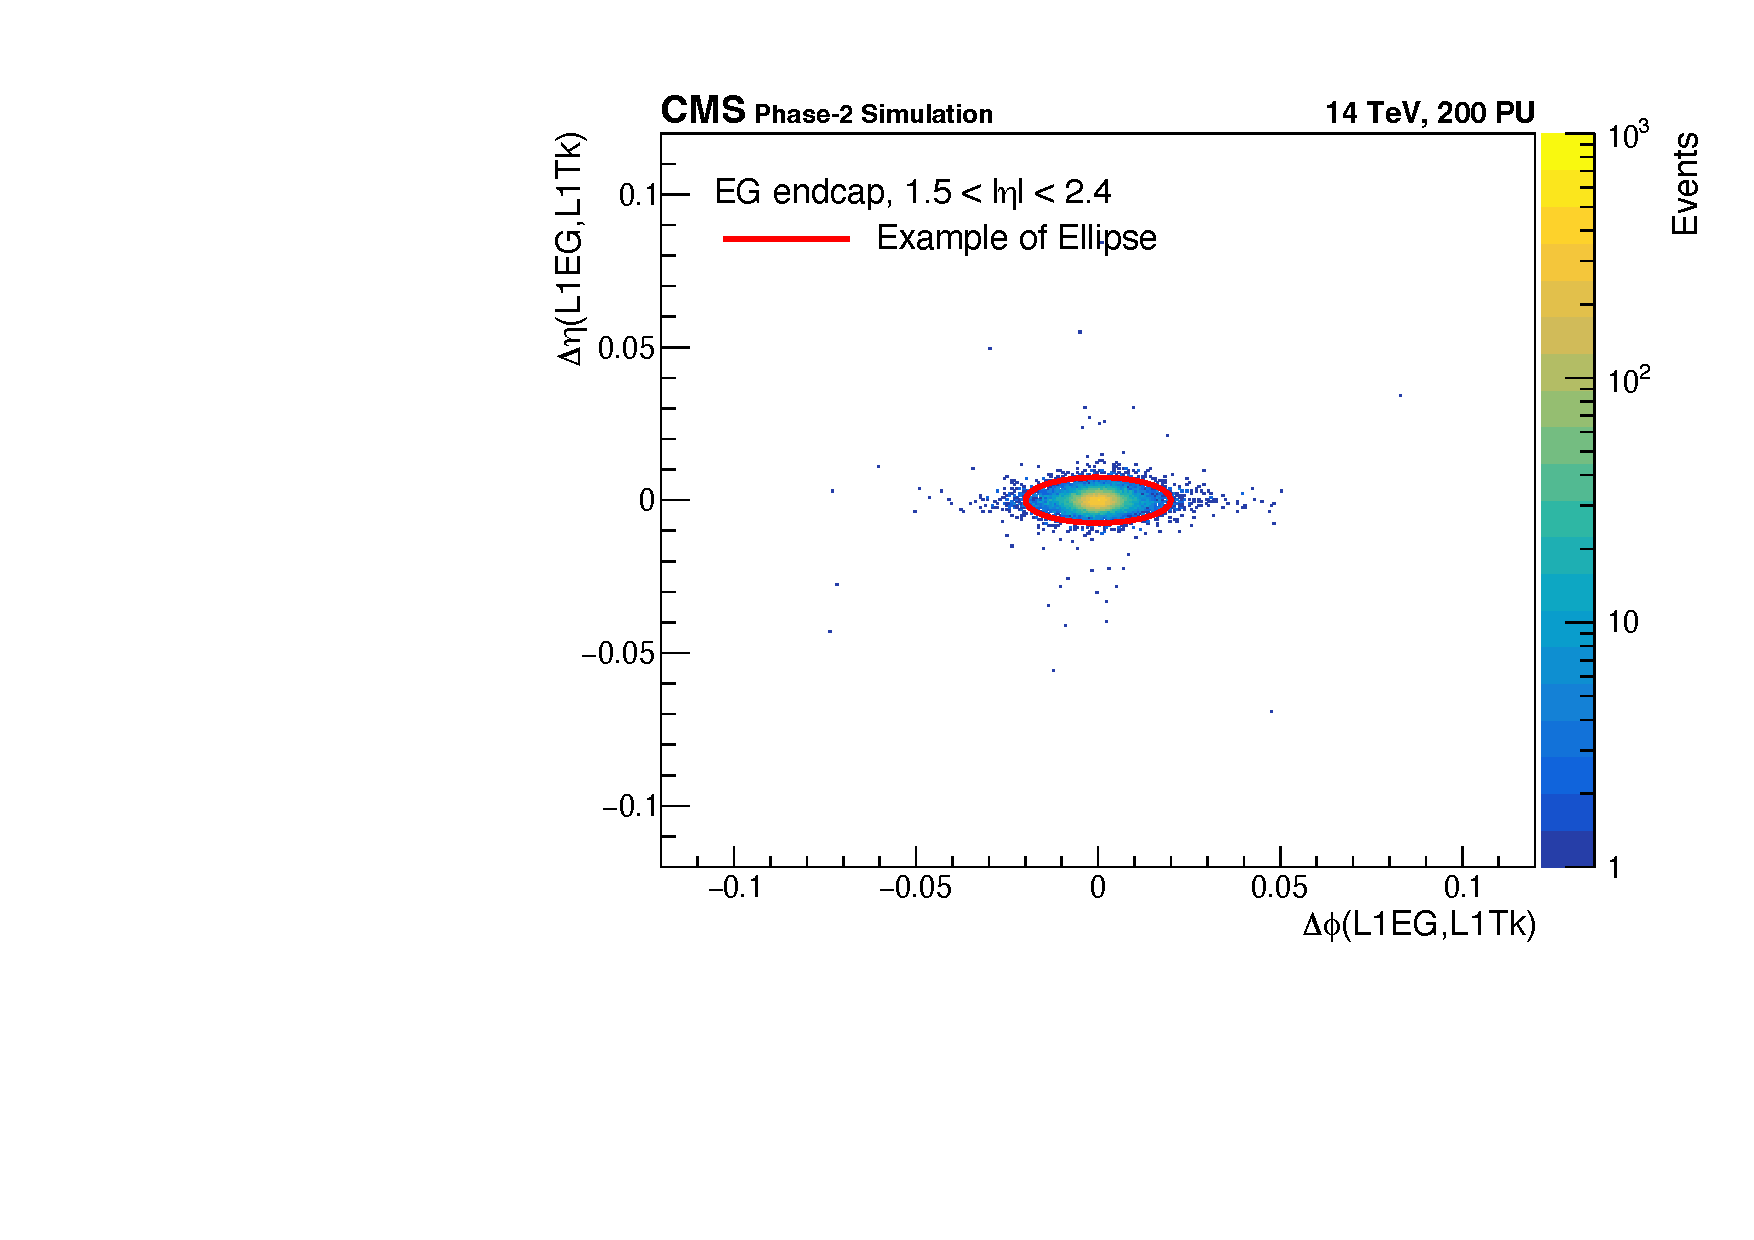
\includegraphics[width=.45\linewidth]{figures/Part2/Upgrade/DR_endcap_new}&
  \end{tabular}
  \caption{(Left) $\mathrm{\Delta}\eta$ vs $\mathrm{\Delta}\phi$ distances between calorimeter clusters and the closest L1 track. (Center) single electron efficiency as a function of the generated $\pt$. The efficiency drop is largely driven by electron track reconstruction which is also reflected in Figure~\ref{fig:trackingperformance}. (Right) trigger rate as a function of the cluster $\pt$.}
 \label{fig:DR_electron}
 \end{center}
\end{figure}

 \begin{figure}[tbh!]
 \begin{center}
  \begin{tabular}{ccc}
   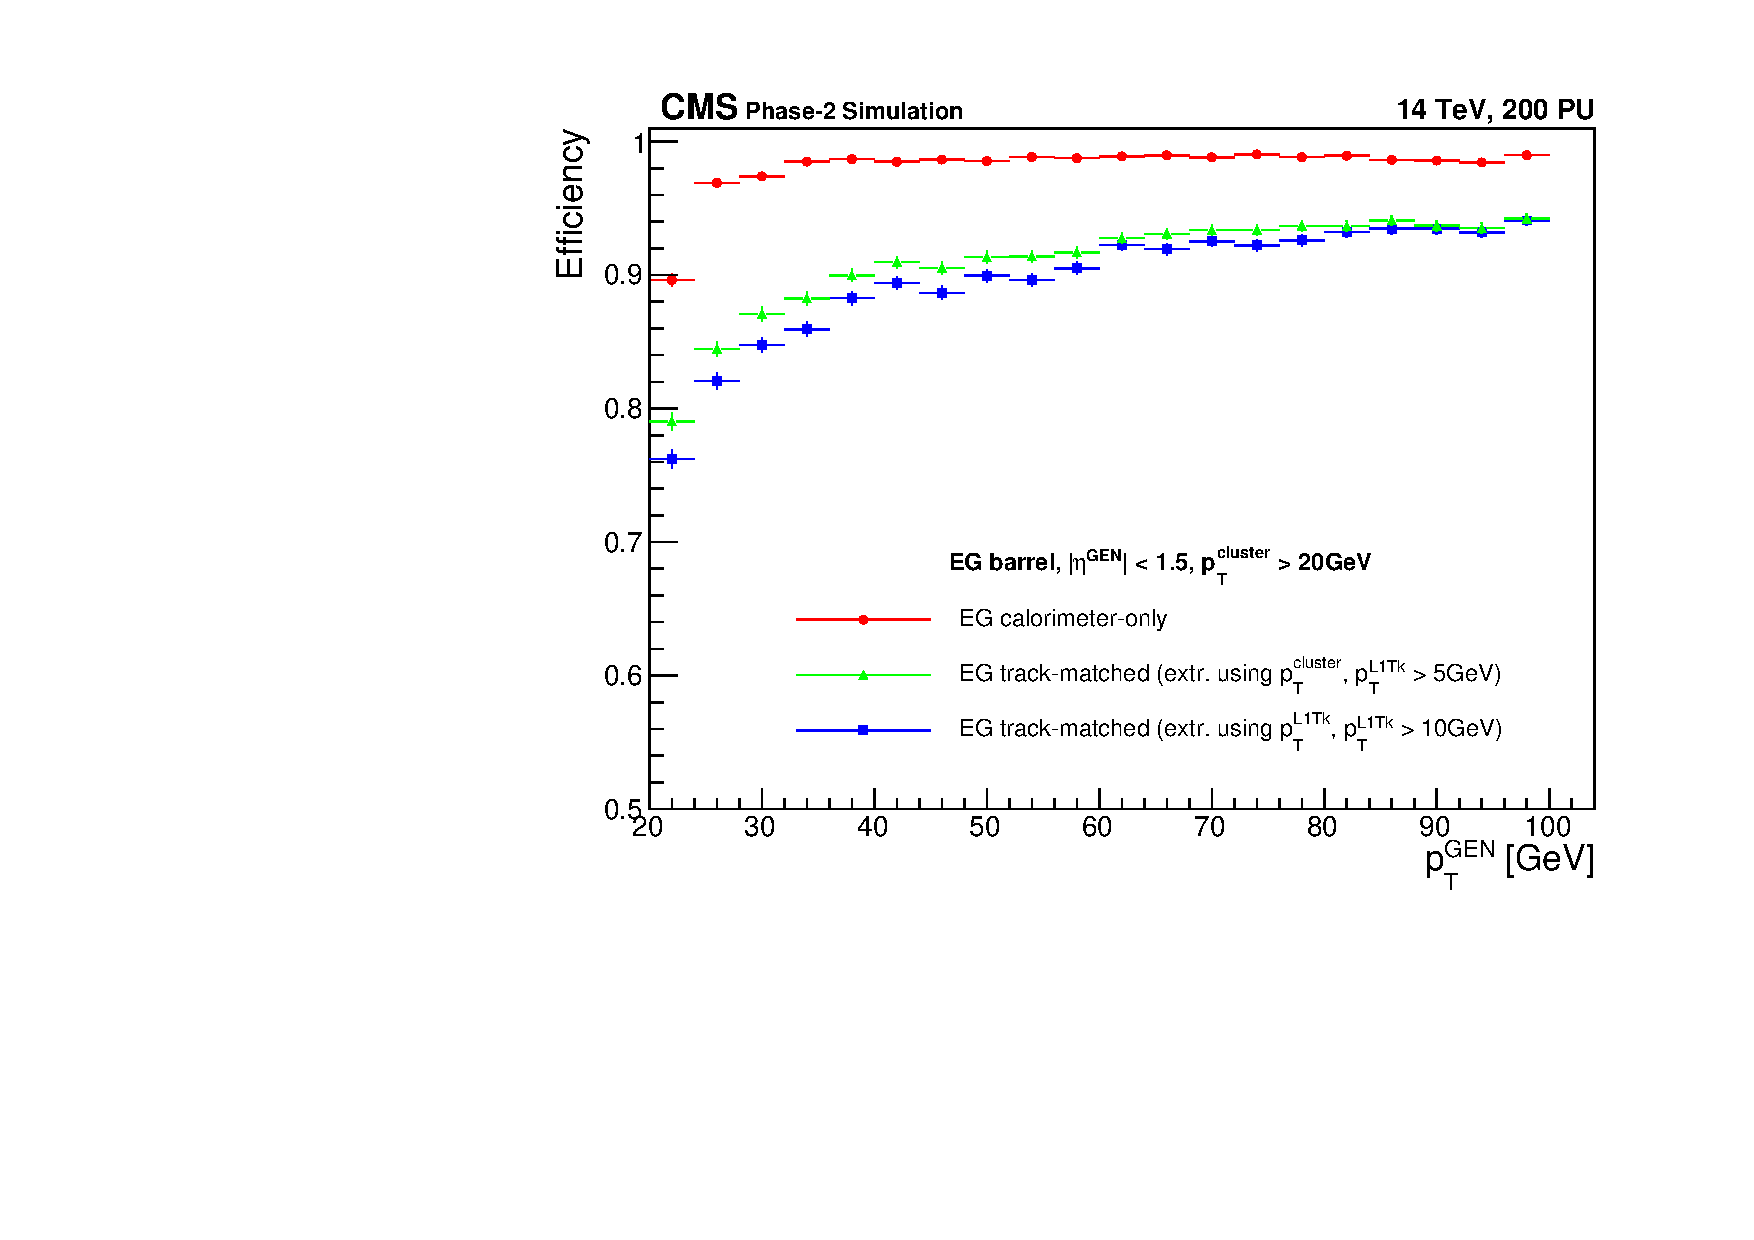
\includegraphics[width=.45\linewidth]{figures/Part2/Upgrade/eff_barrel}&
   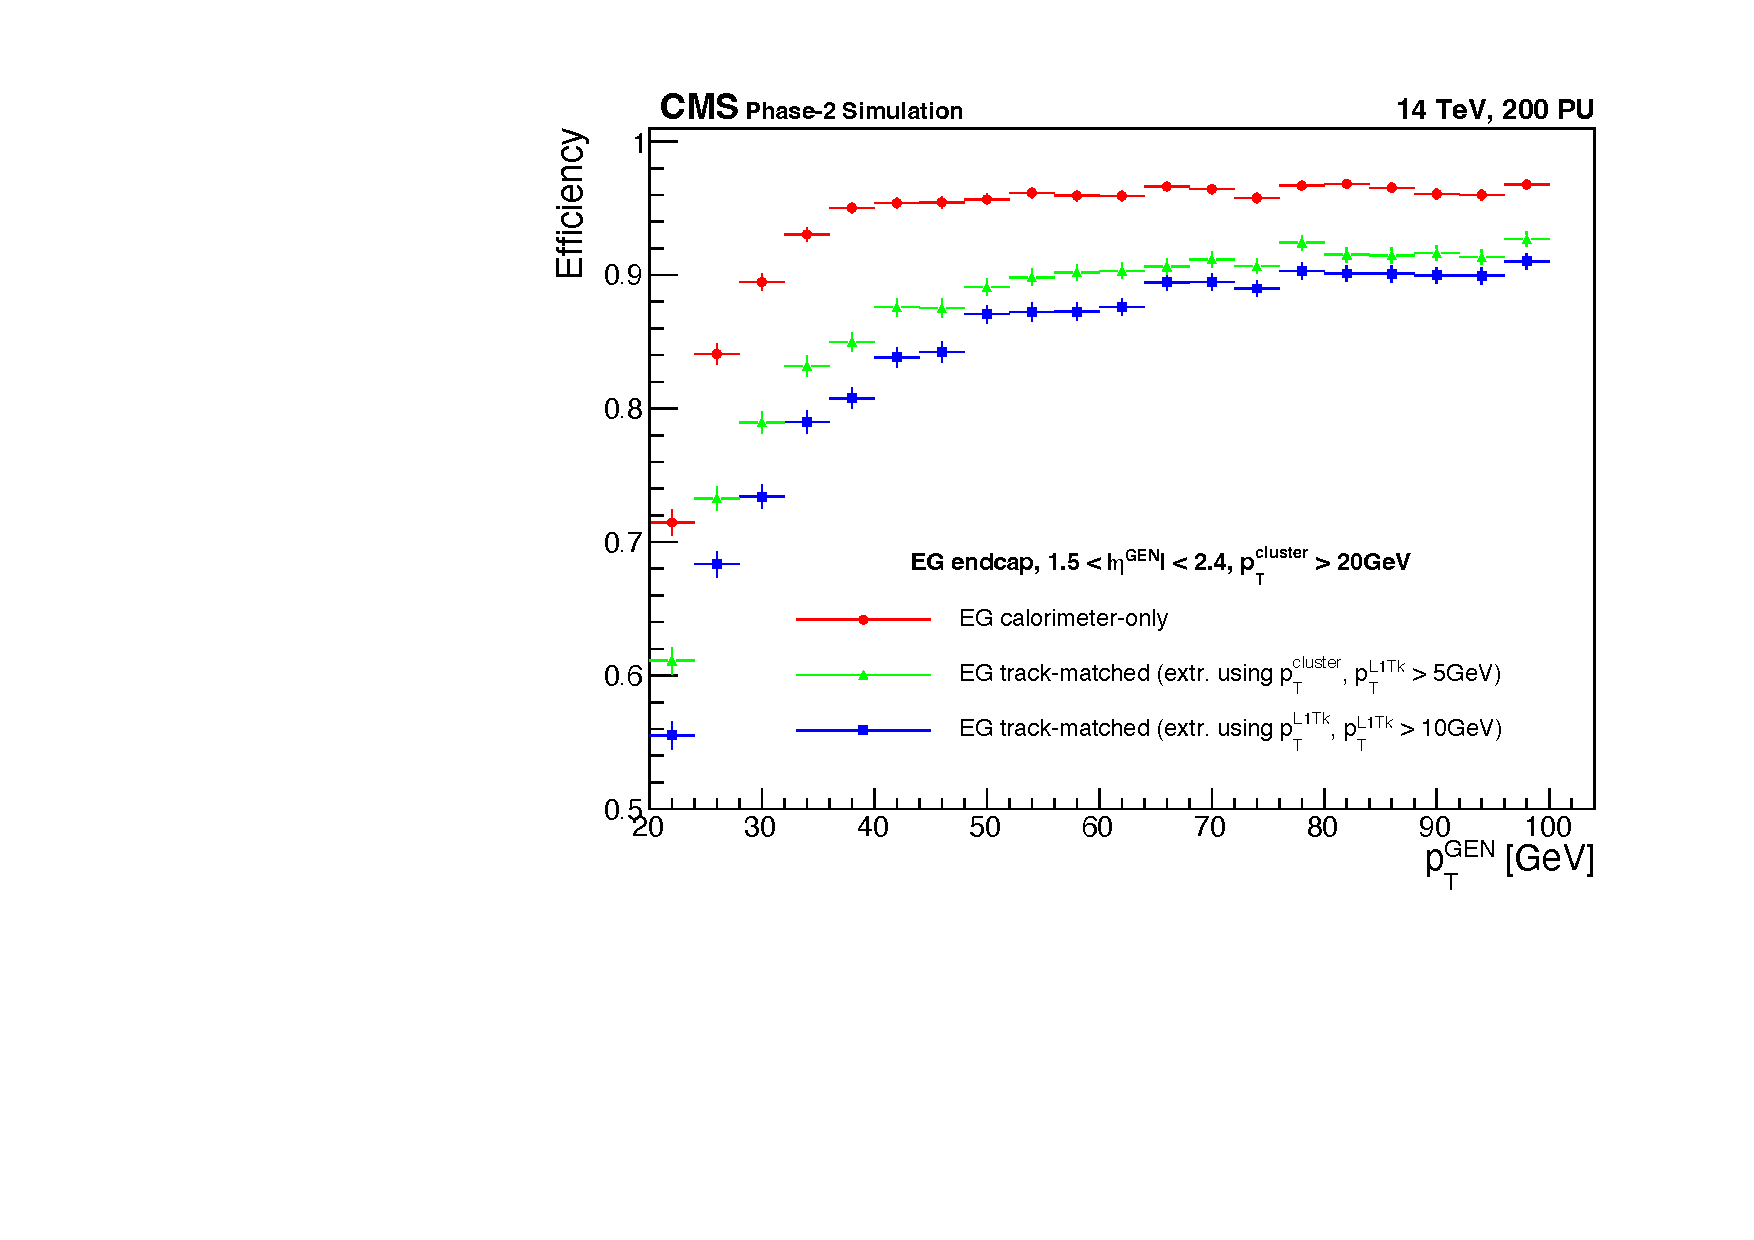
\includegraphics[width=.45\linewidth]{figures/Part2/Upgrade/eff_endcap}&
  \end{tabular}
  \caption{(Left) $\mathrm{\Delta}\eta$ vs $\mathrm{\Delta}\phi$ distances between calorimeter clusters and the closest L1 track. (Center) single electron efficiency as a function of the generated $\pt$. The efficiency drop is largely driven by electron track reconstruction which is also reflected in Figure~\ref{fig:trackingperformance}. (Right) trigger rate as a function of the cluster $\pt$.}
 \label{fig:eff_electron}
 \end{center}
\end{figure}

 \begin{figure}[tbh!]
 \begin{center}
  \begin{tabular}{ccc}
   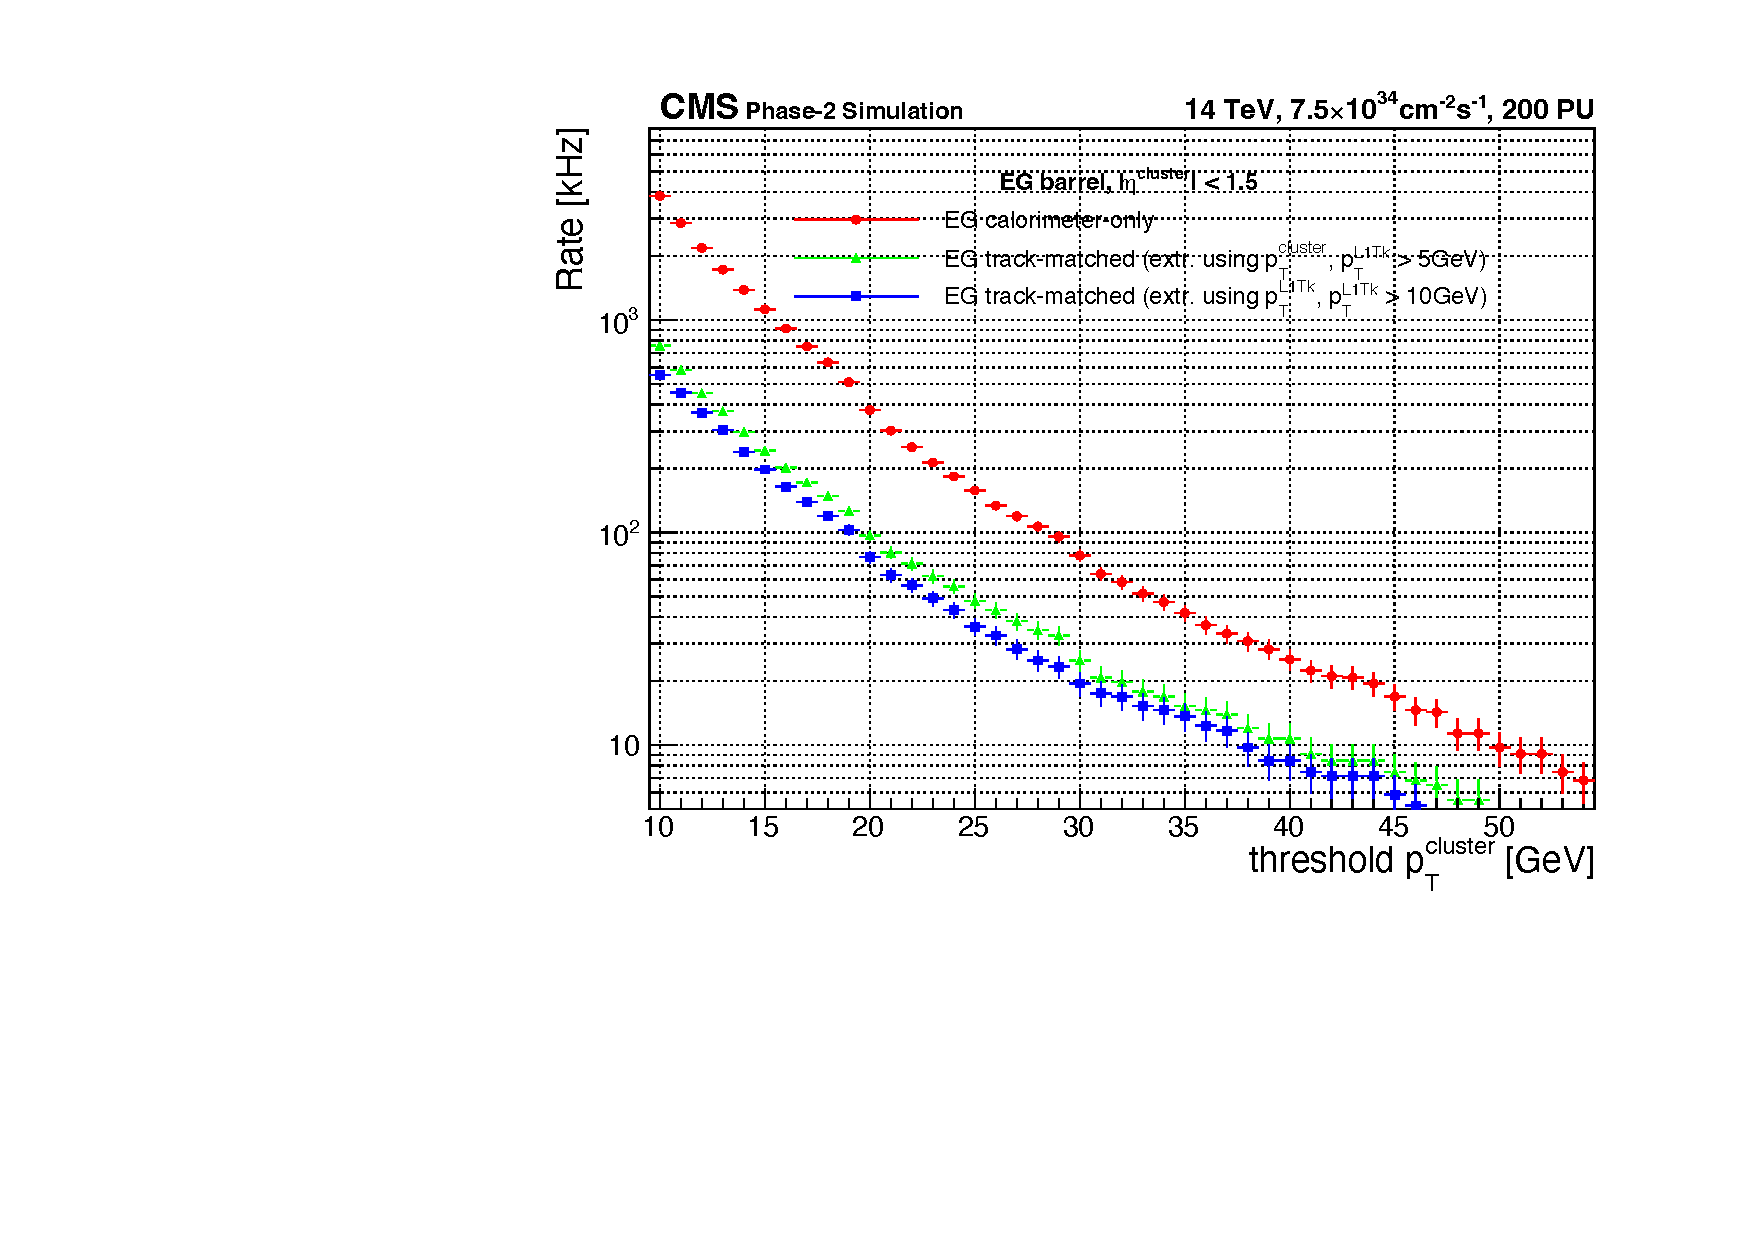
\includegraphics[width=.45\linewidth]{figures/Part2/Upgrade/Rate_barrel}&
   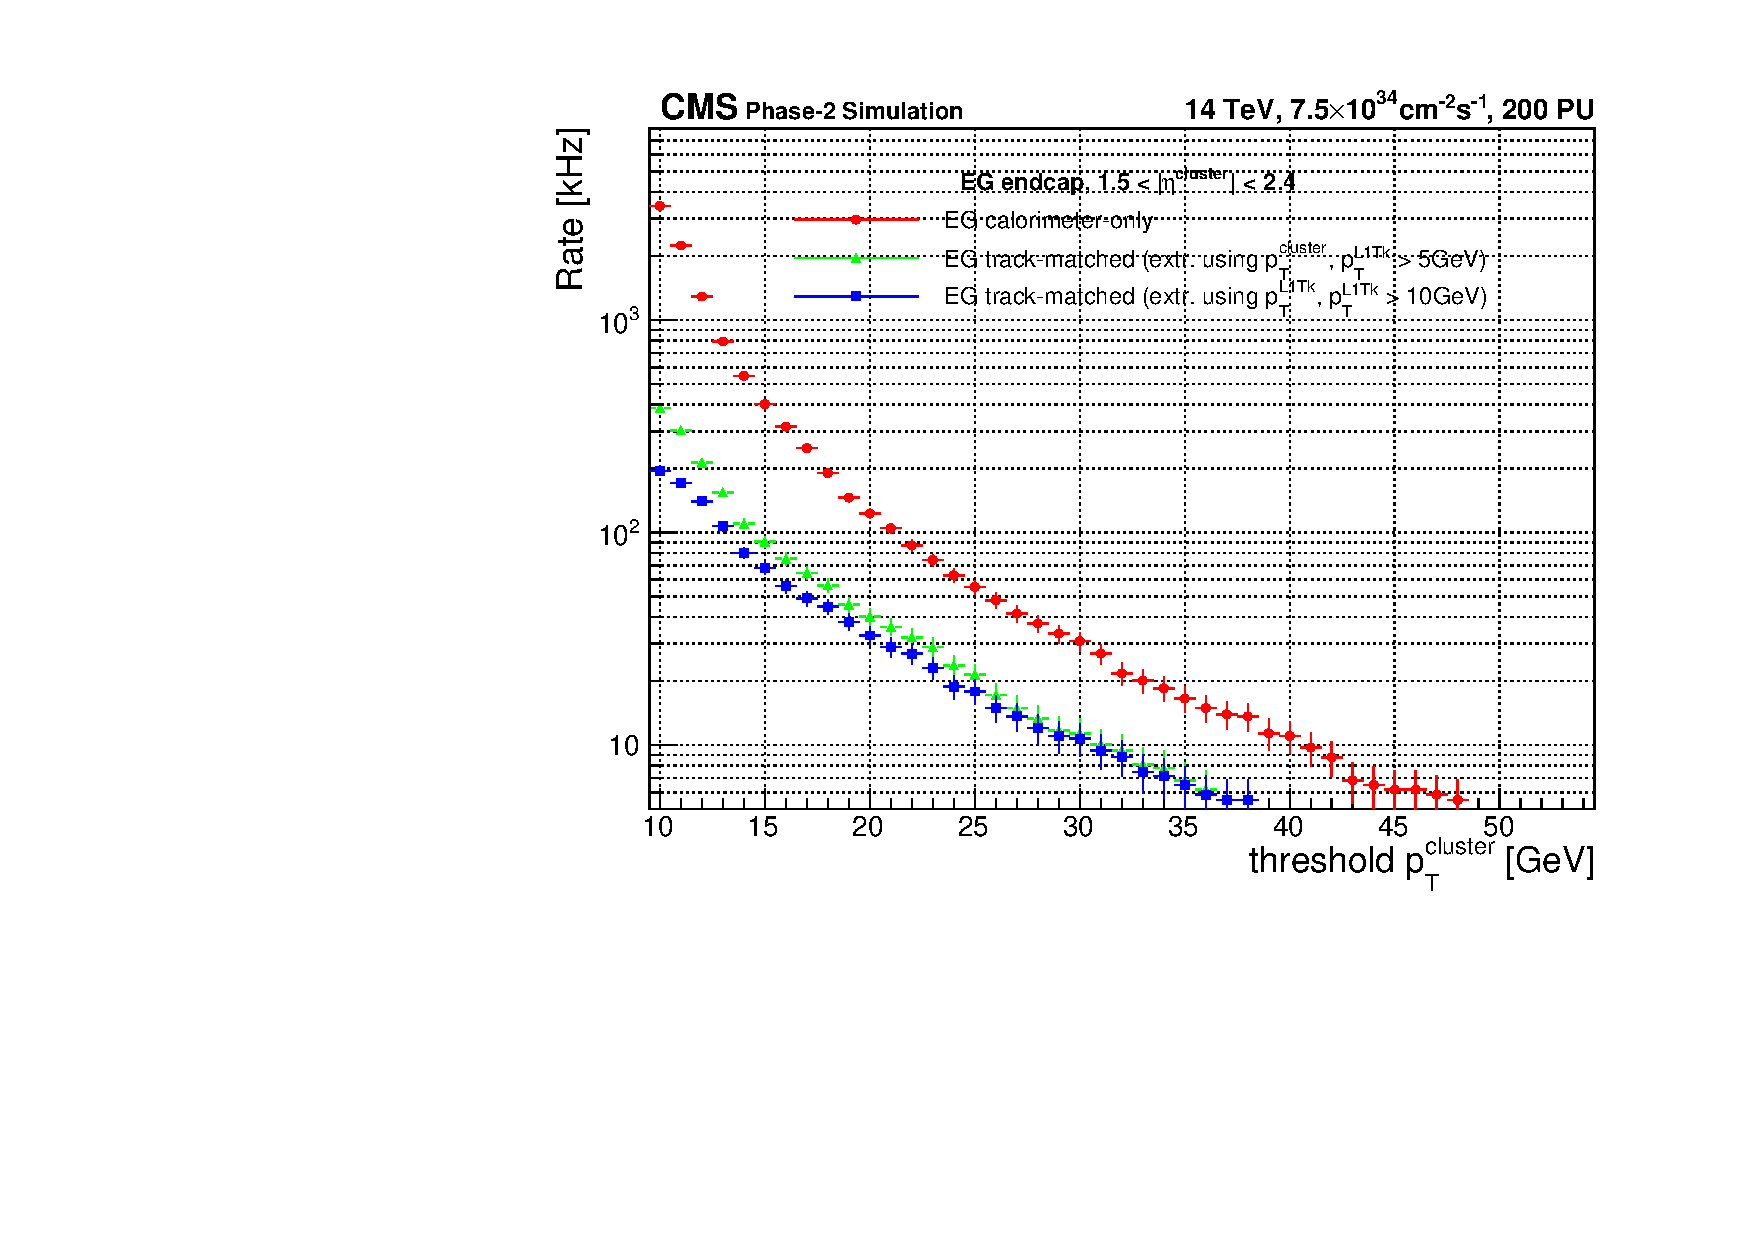
\includegraphics[width=.45\linewidth]{figures/Part2/Upgrade/Rate_endcap}&
  \end{tabular}
  \caption{(Left) $\mathrm{\Delta}\eta$ vs $\mathrm{\Delta}\phi$ distances between calorimeter clusters and the closest L1 track. (Center) single electron efficiency as a function of the generated $\pt$. The efficiency drop is largely driven by electron track reconstruction which is also reflected in Figure~\ref{fig:trackingperformance}. (Right) trigger rate as a function of the cluster $\pt$.}
 \label{fig:rate_electron}
 \end{center}
\end{figure}